\documentclass[oneside]{book}
\usepackage[utf8]{inputenc}
\usepackage{makeidx}
\usepackage{graphicx}
\setcounter{tocdepth}{2}
\usepackage{hyperref}
\hypersetup{pdfborder={0 0 0},colorlinks=false}
\usepackage{verbatim}
\newenvironment{smallverbatim}{\endgraf\small\verbatim}{\endverbatim}
\newenvironment{tinyverbatim}{\endgraf\scriptsize\verbatim}{\endverbatim}
\pagestyle{plain}
\usepackage{float}
\usepackage{pdfpages}
\usepackage{listings}
\usepackage[paperwidth=21.59cm,paperheight=27.94cm]{geometry}
\usepackage{xcolor}


\author{Federico Campoli}
\title{PostgreSQL Database Administration \\ Volume 1 \\ Basic concepts}


\makeindex

\lstdefinestyle{pgsql}{
  belowcaptionskip=1\baselineskip,
  breaklines=true,
  frame=l,
  language=SQL,
  showstringspaces=false,
  basicstyle=\footnotesize\ttfamily,
  keywordstyle=\bfseries\color{green!40!black},
  commentstyle=\itshape\color{purple!40!black},
  identifierstyle=\color{blue},
  stringstyle=\color{orange},
  morekeywords={VACUUM, FULL, ANALYZE, TABLESPACE,SET}
}


\begin{document}
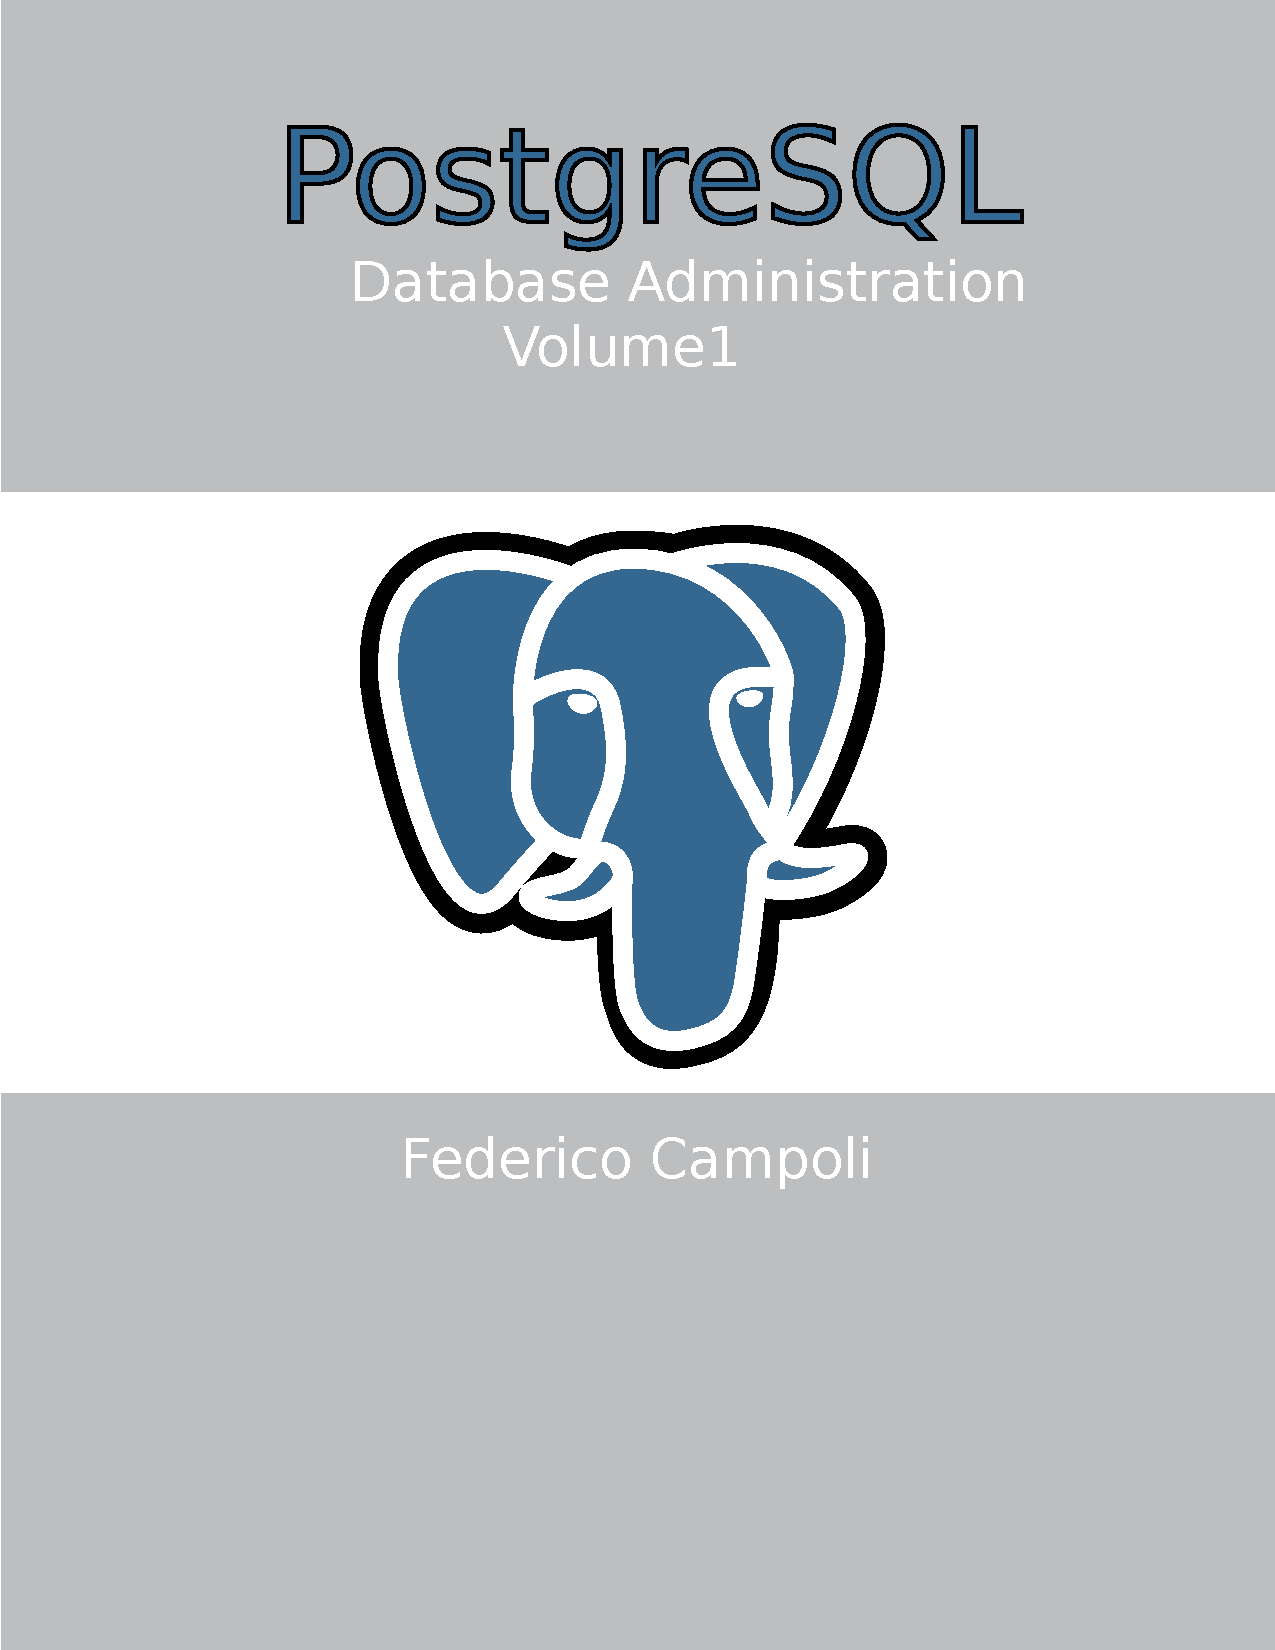
\includepdf{covers/cover_good.pdf}
\maketitle

\newpage{}



\tableofcontents{}

\chapter*{Preface}
When I first came up with the idea to write a PostgreSQL DBA book, my intention was to 
publish it commercially.\newline

Shortly I changed my mind as I became aware the uniqueness of a book for the database 
administrators. Then I decided to keep this book free. The same will happen for the 
next books in this series. I hope this will spread the knowledge on PostgreSQL becoming an 
useful reference.\newline

Just a quick advice before you start reading. I beg your pardon in advance for my 
bad English. Unfortunately I'm not native English and it's very likely the book to be full of 
typos and bad grammar.\newline

However, if you want to help me in cleaning and reviewing the text please to fork 
the github repository where I'm sharing the latex sources 
\href{https://github.com/the4thdoctor/pgdba\_books}{
https://github.com/the4thdoctor/pgdba\_books}.\newline


\section*{Intended audience}
Database administrators, System administrators, Developers

\section*{Book structure}
This book assumes the reader knows how to perform basic user operations such as
connecting to the database and creating tables.\newline

The book covers the basic aspects of database administration from installation
to cluster management.\newline

A couple of chapters are dedicated to the logical and physical structure in
order to show both sides of coin.  The triplet of maintenance backup and restore completes the 
the picture, not exhaustive but good enough to start getting ``hands on'' the product.
The final chapter is dedicated to the developers. The various sections are 
giving advice that can seem quite obvious. But it's better to repeat things than having dangerous 
mistakes when building an application. 

\section*{Version and platform}
This book is based on PostgreSQL version 9.3 running on Debian GNU Linux 7.
References to older versions or different platforms are explicitly specified.

\section*{Thanks}
A big thank you to Craig Barnes for the priceless work on the book review.\newline
The beautiful cover has been made by \href{http://www.bonland.eu/}{
Chiaretta e Bon }.\newline


\chapter{PostgreSQL at glance}
PostgreSQL is a first class product with high end enterprise class features.
This first chapter is a general review on the product with a brief talk on the database's history.

\section{Long time ago in a galaxy far far away...}

Following the works of the Berkeley's Professor  Michael Stonebraker, in 1996
Marc G. Fournier\index{Marc G. Fournier} asked for any volunteers interested
in revamping the Postgres 95 project.

\framebox{\parbox[t][1\totalheight]{1\columnwidth}{%
{\scriptsize Date: Mon, 08 Jul 1996 22:12:19-0400 (EDT) From: \char`\"{}Marc
G. Fournier\char`\"{} <scrappy@ki.net> }{\scriptsize \par}

{\scriptsize Subject: {[}PG95]: Developers interested in improving
PG95? }{\scriptsize \par}

{\scriptsize To: Postgres 95 Users <postgres95@oozoo.vnet.net> }{\scriptsize \par}

{\scriptsize Hi... A while back, there was talk of a TODO list and
development moving forward on Postgres95 ... }{\scriptsize \par}

{\scriptsize at which point in time I volunteered to put up a cvs
archive and sup server so that making updates (and getting at the
\char`\"{}newest source code\char`\"{}) was easier to do... }{\scriptsize \par}

{\scriptsize ... Just got the sup server up and running, and for those
that are familiar with sup, the following should work (ie. I can access
the sup server from my machines using this): }{\scriptsize \par}

{\scriptsize ...............}%
}}%

The answer came from Bruce Momjian\index{Bruce Momjian},Thomas
Lockhart\index{Thomas Lockhart}, and Vadim Mikheev\index{Vadim Mikheev}, the very
first PostgreSQL Global Development Team.

\section{Features}
Every time a new major release is published, new powerful features join the
rich feature set.
Here's a small excerpt of what the latest version offers in terms of flexibility
and reliability.

\subsection{Write ahead logging}
Like any standards compliant RDBMS, PostgreSQL implements a write ahead log.
In short, when a data block is updated the change is saved in a reliable
location, the so called write ahead log\index{wal}\index{write ahead log}. The
effective write on the data file is performed later. Should the database crash
the WAL is scanned and the saved blocks are replayed during the
crash recovery. PostgreSQL stores the redo records in fixed size segments,
usually 16 MB. When the wal segment is full PostgreSQL switches to a newly
created or recycled wal segment in the process called log switch. \index{log
switch}

\subsection{Point in time recovery}
\index{pitr}\index{point in time recovery}\index{log shipping}When the
log switch happens it is possible to archive the previous segment in a safe
location. Taking an inconsistent copy of the data directory is possible to
restore a fully functional cluster because the archived wal segments have all
the information to replay the physical data blocks on the inconsistent data
files. The restore can be, optionally stopped at a given point in time. For
example is possible to recover a PostgreSQL cluster to one second before the
a catastrophic happening (e.g. a table drop).

\subsection{Standby server and high availability}
\index{standby server}\index{high availability}The inconsistent snapshot
can be configured to stay up in continuous archive recovery. PostgreSQL 8.4
supports the warm standby\index{warm standby} configuration where the standby
server does not accept connections. From version 9.0 it is possible to enable
hot standby\index{hot standby} configuration to access the standby server in
read only mode.

\subsection{Streaming replication}
The wal archiving doesn't work in real time. The wal shipping happens only
after the log switch and in a low activity server this can leave the standby
behind the master for a while. Using the streaming replication\index{streaming
replication} a standby server can get the wal blocks over a database connection
in almost real time.


\subsection{Transactions}
PostgreSQL fully supports transactions and is ACID compliant.
Version 8.0 introduced save points.

\subsection{Procedural languages}
PostgreSQL has it's own feature rich procedural language pl/pgsql, but many procedural
languages such as perl or python are available for writing database functions.
The DO keyword was introduced in version 9.1 to allow anonymous function code
blocks.

\subsection{Partitioning}
The partitioning\index{partitioning}\index{constraint exclusion} implementation in
PostgreSQL is still very basic. Partitions are tables connected with one
empty parent table using table inheritance.

By defining check constraints on the partitioned data, the database can
exclude partitions from a query on the parent table based on the WHERE
clause criteria.

As the physical storage is distinct for each partition, no global primary key
enforcement nor foreign key constraints can be defined on the partitioned
structure.

\subsection{Cost based optimiser}
The cost based optimiser, or CBO,\index{cost based optimizer}\index{CBO} is
one of PostgreSQL's strong points.
The query execution plan is dynamically determined and self adapting to the
underlying data structure or the estimated amount of data affected.
PostgreSQL also supports the genetic query optimizer GEQO.

\subsection{Multi platform support}
PostgreSQL\index{platform} nowadays supports almost any unix flavour, and from
version 8.0 is native to Windows.

\subsection{Tablespaces}
Tablespace support permits fine grained distribution of the data files across
filesystems.

\subsection{MVCC}
The way PostgreSQL keeps things consistent is the MVCC which stands for Multi
Version Concurrency Control. The mechanism is neat and efficient, offering
great advantages and one single disadvantage. We'll see in detail later but
keep in mind this important sentence. \\
There's no such thing as an update in PostgreSQL.

\subsection{Triggers} TODO
Triggers to execute automated tasks on when DML is performed on tables and also
views are supported at any level. The events triggers are also supported.

\subsection{Views}
The read only views are well consodlidated in PostgreSQL.
In the version 9.3 was added the support for the materialized and updatable.
Also the implementation is still very basic as no incremental refresh for the
mat views nor update is possible on complex views. Anyway is still possible to
replicate this behaviour using the triggers and procedures.

\subsection{Constraint enforcement}
PostgreSQL supports primary keys and unique keys to enforce local data meanwhile
the referential integrity is guaranteed with the foreign keys.
The check constraint to validate custom data sets is also supported.

\subsection{Extension system}
PostgreSQL implements the extension system. Almost all the previously known
contrib modules are now implemented in this efficient way to add feature to the
server using a simple SQL command.

\chapter{Database installation}
\label{cha:DB_INSTALL}
In this chapter will see how to install PostgreSQL on Debian Gnu Linux. We'll take a look to 
two procedures, compiling from source and using the packages shipped by the pgdg 
\index{pgdg apt repository} apt repository.\newline 
There are advantages and disadvantages on both procedures. The compile from source offers a fine
grain control on all the aspects of the binaries configuration. Also doesn't have risks of
unwanted restarts when upgrading and it's possible to install and upgrade the binaries with normal
privileges.\newline

The packaged install is easier to manage when deploying the new binaries on the server, in
particular if there is a large number of installations to manage. The binary packages are
released shortly after a new update is released. Because the frequency for the minor
releases is not fixed, it could happen to have in place bugs affecting the production for months.
For example the bug causing the standby server crashing when the master found invalid pages during
a conventional vacuum, it was fixed almost immediately. Unfortunately the release with the fix
appeared after five months.\newline


\section{Install from source}
Using the configure script with the default settings requires the root access when installing.
That's because the permissions in the target location /usr/local don't allow the write for normal
users. This method adopts a different install location and requires the root access only for the os
user creation and the dependencies install. 
Before starting the PostgreSQL part ask your sysadmin to run the following commands.

\begin{itemize}

 \item useradd -d /home/postgres -s /bin/bash -m -U postgres
 \item passwd postgres 
 \item apt-get update
 \item apt-get install build-essential  libreadline6-dev  zlib1g-dev
\end{itemize}

Please note the second step will require inserting a new user password. Unless is a personal
test it's better to avoid obvious passwords like \textit{postgres}.\newline

In order to build the binaries we must download and extract the PostgreSQL's source tarball.

\begin{verbatim}
mkdir ~/download
cd ~/download
wget http://ftp.postgresql.org/pub/source/v9.3.5/postgresql-9.3.5.tar.bz2
tar xfj postgresql-9.3.5.tar.bz2
cd postgresql-9.3.5
\end{verbatim}


Using the configure script's option --prefix we'll point the install directory to a writable
location. We can also use a director named after the the major version's numbering. This will allow
us to have installed different PostgreSQL versions without problems.

\begin{verbatim}
mkdir -p /home/postgres/bin/9.3
./configure --prefix=/home/postgres/bin/9.3
\end{verbatim}

The configuration script will check all the dependencies and, if there's no error, will generate 
the makefiles. Then we can start the build simply running the command \textit{make}. The time
required for compiling is variable and depends from the system's power. If you have a multicore
processor the make -j option can improve significantly the build time. When the build is is complete
it's a good idea to to run the regression tests. Those tests are designed to find any regression or
malfunction before the binaries are installed.

\begin{verbatim}
make
<very verbose output>

make check 

\end{verbatim}

The test's results are written in the source's subdirectory src/test/regress/results. If
there's no error we can finalise the installation with the command make install.

\begin{verbatim}
make install
\end{verbatim}

This will create into the folder /home/postgres/bin/9.3 four subfolders \textit{bin} 
\textit{include} \textit{lib} and \textit{share}.

\begin{itemize}
 \item \textbf{bin} is the location for PostgreSQL's binaries
 \item \textbf{include} contains the server's header files
 \item \textbf{lib} is the location where to put the shared libraries
 \item \textbf{share} is where the example files and the extension configurations are stored
\end{itemize}


\section{Packaged install}
\label{sec:DEBIAN_INSTALL}

The PostgreSQL Global Development Group manages a repository in order to facilitate the
installations on the Linux distributions based on the debian's packaging system. 

Currently the supported distributions are

\begin{itemize}
 \item Debian 6.0 (squeeze)
 \item Debian 7.0 (wheezy)
 \item Debian unstable (sid) 
 \item Ubuntu 10.04 (lucid)
 \item Ubuntu 12.04 (precise)
 \item Ubuntu 13.10 (saucy)
 \item Ubuntu 14.04 (trusty) 
\end{itemize}

The PostgreSQL's versions available are 
\begin{itemize}
 \item PostgreSQL 9.0 
 \item PostgreSQL 9.1 
 \item PostgreSQL 9.2 
 \item PostgreSQL 9.3
 \item PostgreSQL 9.4
\end{itemize}

The he packages are available either for amd64 and i386 architecture.

Anyway, the up to date list is available on the the wiki page 
\href{http://wiki.postgresql.org/wiki/Apt}{http://wiki.postgresql.org/wiki/Apt}.\newline

All the installation steps require root privileges, via sudo or acquiring the root login via su.
Before starting configuring the repository it's a good idea to import the GPG key for the
package validation.

In a root shell simply run
\begin{verbatim}
wget --quiet -O - https://www.postgresql.org/media/keys/ACCC4CF8.asc | sudo apt-key add -
\end{verbatim}
When the key is imported create a file named pgdg.list into the directory /etc/apt/sources.d/ and
add the following row.

\begin{verbatim}
deb http://apt.postgresql.org/pub/repos/apt/ {codename}-pgdg main
\end{verbatim}


The distribution's codename can be found using the command lsb\_release -c. 
e.g.
\begin{verbatim}
thedoctor@tardis:~$ lsb_release -c
Codename:       wheezy
\end{verbatim}

After the repository configuration the installation is completed with two simple commands.

\begin{verbatim}
apt-get update
apt-get install postgreql-9.3 postgreql-contrib-9.3 postgreql-client-9.3 
\end{verbatim}

Be aware that this method, as automated installation task creates a new database cluster in
the default directory /var/lib/postgresql.


\chapter{Install structure}\label{cha:INSTALLSTRUCT}
Depending on the installation method, the install structure is set up in a single directory or 
in multiple folders.\newline

The install from source creates into the target directory four subfolders \textit{bin} 
\textit{include} \textit{lib} and \textit{share}.

\begin{itemize}
 \item \textbf{bin} is the location for PostgreSQL's binaries
 \item \textbf{include} contains the server's header files
 \item \textbf{lib} is the location where to put the shared libraries
 \item \textbf{share} is where the example files and the extension configurations are stored
\end{itemize}


The packaged install puts the binaries and the libraries in the folder /usr/lib/postgresql 
organised by major version. For example the 9.3 install will put the binaries into 
/usr/lib/postgresql/9.3/bin and the libraries in /usr/lib/postgresql/9.3/lib. The extensions and 
contributed modules are installed into the folder /usr/share/postgresql with the same structure. In 
the directory /usr/bin/ are installed the debian's specific utilities and the symbolic link psql 
pointing the file /usr/lib/share/postgresql-common/pg\_wrapper. This file is a perl script which 
calls the PostgreSQL client reading the version the cluster and the default database from the file 
~/.postgresqlrc or in /etc/postgresql-common/user\_clusters.\newline


\section{The core binaries}
The PostgreSQL binaries can be split in two groups, the core and the wrappers alongside with the 
contributed modules. Let's start then with the former group.

\subsection{postgres}\index{postgres}
\label{sec:POSTGRES}
This is the PostgreSQL's main process. The program can be started directly or using the pg\_ctl 
utility. The second method is to be preferred as offer a simpler way to control the postgres 
process. The direct execution is the unavoidable choice when the database won't start for an old XID 
near to the wraparound failure\index{XID wraparound failure}. 
In this case the cluster can only start in single user mode to perform a cluster wide vacuum. For 
historical reasons there's also a symbolic link named postmaster pointing to the postgres 
executable.

\subsection{pg\_ctl}\index{pg\_ctl}
\label{sub:PGCTL}
This utility is the simplest way for managing a PostgreSQL instance. The program reads the postgres 
pid from the cluster's data area and sending the os signals manages the start the stop or the 
process reload. It's also possible to send kill signals to the running instance. 
The pg\_ctl The supported actions are the following.

\begin{itemize}
 \item \textbf{init[db]} initialises a directory as PostgreSQL data area
 \item \textbf{start} starts a PostgreSQL instance
 \item \textbf{stop} shutdowns a PostgreSQL instance
 \item \textbf{reload} reloads the configuration's files
 \item \textbf{status} checks the PostgreSQL instance running status
 \item \textbf{promote} promotes a standby server 
 \item \textbf{kill} sends a custom signal to the running instance
\end{itemize}

In \ref{cha:MANAGING} we'll se how to manage the cluster.

\subsection{initdb}\index{initdb}
Is the binary which initialises the PostgreSQL data area. The directory to initialise must 
be empty. Various options can be specified on the command line, like the character enconding or the 
collation order. 

\subsection{psql}\index{psql}
This is the PostgreSQL command line client. The client it looks very essential, however is one of 
the most flexible tools available to interact with the server and the only choice when working on 
the command line.

\subsection{pg\_dump}\index{pg\_dump}
\label{sub:PGDUMP}
This is the binary dedicated to the backup. Can produce consistent backups in various formats. The 
usage is described shown in \ref{cha:BACKUP}.

\subsection{pg\_restore}\index{pg\_restore}
This program is used to restore a database reading a binary dump like the custom or directory 
format. It's able to run the restore in multiple jobs in order to speed up the process. The usage 
is described in \ref{cha:RESTORE}

\subsection{pg\_controldata}\index{pg\_controldata}\label{sub:PGCONTROLDATA}
This program can query the cluster's control file where PostgreSQLstores critical informations for 
the cluster activity and reliability. 

\subsection{pg\_resetxlog}\index{pg\_resetxlog}
If a WAL file becomes corrupted the cluster cannot perform a crash recovery. This lead to a not 
startable cluster in case of system crash. In this catastrophic scenario there's still a 
possibility to start the cluster. Using pg\_resetxlog the cluster is cleared of any WAL file, the  
control file is initialised from scratch and the transaction's count is restarted.\newline

The \textit{tabula rasa} have a cost indeed. The cluster lose any reference between the 
transactions progression and the data files. The physical integrity is lost and any attempt to run 
queries which write data will results in corruption.\newline 

The PostgreSQL's documentation is absolutely clear on this point.

\begin{verbatim}

After running pg_resetxlog the database must start without user access, 
the entire content must be dumped, the data directory must be dropped and recreated 
from scratch using initdb and then the dump file can be restored using psql or pg_restore
\end{verbatim}

\section{Wrappers and contributed modules}
The second group of binaries is composed by the contributions and the wrappers. The 
contributed modules add functions otherwise not available. The wrappers add command line 
functions already present as SQL statements. Someone will notice the lack of HA specific binaries 
like pg\_receivexlog and pg\_archivecleanup. They have been purposely skipped because beyond the 
scope of this book.

\subsection{The create and drop utilities}
The  binaries with the prefix create and drop like, createdb createlang createuser and dropdb, 
droplang, dropuser, are wrappers for the corresponding SQL functions. Each program performs the 
creation and the drop action on the corresponding named object. For example createdb adds a 
database to the cluster and dropdb will drop the specified database. 

\subsection{clusterdb}\index{clusterdb}
This program performs a database wide cluster on the tables with clustered indices. 
The binary can run on a single table specified on the command line. In \ref{sec:VACFULL} we'll 
take a look to CLUSTER and VACUUM FULL.

\subsection{reindexdb}\index{reindexdb}
The command does a database wide reindex. It's possible to run the command just on a table or index 
passing the relation's name on the command line. In \ref{sec:REINDEX} we'll take a good look to 
the index management.

\subsection{vacuumdb}\index{vacuumdb}
This binary is a wrapper for the VACUUM \index{VACUUM} SQL command. This is the most important 
maintenance task and shouldn't be ignored. The program performs a database wide VACUUM if executed 
without a target relation. Alongside with a common vacuum it's possible to have the usage 
statistics updated on the same time.

\subsection{vacuumlo}\index{vacuumlo}
This binary will remove the orphaned large objects from the pg\_largeobject system table. The 
pg\_largeobject is used to store the binary objects bigger than the limit of 1GB imposed by the 
bytea data type. The limit for a large object it is 2 GB since the version 9.2. From the version 
9.3 the limit was increased to 4 TB. 

\section{Debian's specific utilities}
Finally let's take a look to the debian's specific utilities. They are a collection of perl scripts 
used to simplify the cluster's management. Their install location is /usr/bin mostly like symbolic 
links to the actual executable. We already mentioned one of them in the chapter's introduction, the 
psql pointing to the pg\_wrapper PERL script.

\subsection{pg\_createcluster}\index{pg\_createcluster}
This script adds a new PostgreSQL cluster with the given major version, if installed, and the 
given name. The script puts all the configurations in /etc/postgresql. Each major version have a 
dedicated directory under which is present a group of directories with the cluster's specific 
configuration files. If not specified the data directory is created into the folder 
/var/lib/postgresql. It's also possible to specify the options for initd.

\subsection{pg\_dropcluster}\index{pg\_dropcluster}
The program delete a PostgreSQL cluster created previously with pg\_createcluster. The 
program will not drop a running cluster. If the dropped cluster have any tablespace those must be 
manually removed after the drop as the program doesn't follow the symbolic links.

\subsection{pg\_lscluster}\index{pg\_lscluster}
Lists the clusters created with pg\_createcluster.

\subsection{pg\_ctlcluster}\index{pg\_ctlcluster}
\label{sub:PGCTLDEB}
The program manages the cluster in a similar way pg\_ctl does. 
Before the version 9.2 this wrapper had a dangerous behaviour for the shutdown. The script did not 
offered a flexible way to provide the shutdown mode. More informations about the shutdown 
sequence are in \ref{sec:SHUTDOWN_SEQ}. 
Without any option pg\_ctlcluster performs a smart shutdown mode.
The --force option tells the script to try a \textit{fast} shutdown mode. Unfortunately if the 
database doesn't shutdown in a \textit{reasonable time} the script performs an \textit{immediate} 
shutdown. After another short wait, if the the instance is still up the script sends a 
\textit{kill -9} to the postgres process. Because this kind of actions can result in data loss  
they should be made manually by the DBA. It's better to avoid the shutdown using pg\_ctlcluster.

\chapter{Managing the cluster}
\label{cha:MANAGING}
A PostgreSQL cluster is made of two components. A physical location initialised as data area 
and the postgres process attached to a shared memory segment, the shared buffer. The debian's 
package's installation, automatically set up a fully functional PostgreSQL cluster in the directory 
/var/lib/postgresql. This is good because it's possible to explore the product immediately.
However, 
it's not uncommon to find clusters used in production with the minimal default configuration's 
values, just because the binary installation does not make it clear what happens \textit{under the 
bonnet}.

This chapter will explain how a PostgreSQL cluster works and how critical is its 
management. 

\section{Initialising the data directory}

The data area is initialised by initdb\index{initdb}. The program requires an empty directory to 
write into to successful complete. Where the initdb binary is located depends from the installation 
method. We already discussed of this in \ref{cha:INSTALLSTRUCT} and \ref{cha:DB_INSTALL}. 

The accepted parameters for customising cluster's data area are various. Anyway, running 
initdb without parameters will make the program to use the value stored into the environment 
variable PGDATA. If the variable is unset the program will exit without any further action.\newline

For example, using the initdb shipped with the debian archive requires the following commands.

\begin{verbatim}
postgres@tardis:~/$ mkdir tempdata
postgres@tardis:~/$ cd tempdata
postgres@tardis:~/tempdata$ export PGDATA=`pwd`
postgres@tardis:~/tempdata$ /usr/lib/postgresql/9.3/bin/initdb 
The files belonging to this database system will be owned by user "postgres".
This user must also own the server process.

The database cluster will be initialized with locale "en_GB.UTF-8".
The default database encoding has accordingly been set to "UTF8".
The default text search configuration will be set to "english".

Data page checksums are disabled.

fixing permissions on existing directory /var/lib/postgresql/tempdata ... ok
creating subdirectories ... ok
selecting default max_connections ... 100
selecting default shared_buffers ... 128MB
creating configuration files ... ok
creating template1 database in /var/lib/postgresql/tempdata/base/1 ... ok
initializing pg_authid ... ok
initializing dependencies ... ok
creating system views ... ok
loading system objects' descriptions ... ok
creating collations ... ok
creating conversions ... ok
creating dictionaries ... ok
setting privileges on built-in objects ... ok
creating information schema ... ok
loading PL/pgSQL server-side language ... ok
vacuuming database template1 ... ok
copying template1 to template0 ... ok
copying template1 to postgres ... ok
syncing data to disk ... ok

WARNING: enabling "trust" authentication for local connections
You can change this by editing pg_hba.conf or using the option -A, or
--auth-local and --auth-host, the next time you run initdb.

Success. You can now start the database server using:

    /usr/lib/postgresql/9.3/bin/postgres -D /var/lib/postgresql/tempdata
or
    /usr/lib/postgresql/9.3/bin/pg_ctl -D /var/lib/postgresql/tempdata -l 
logfile start

\end{verbatim}

PostgreSQL 9.3 introduces\index{checksums, data page}\index{data page checksums} the data page 
checksums used for detecting the data page corruption. This great feature can be enabled only when 
initialising the data area with initdb and is cluster wide. The extra overhead caused by the 
checksums is something to consider because the only way to disable the data checksums is a dump 
and reload on a fresh data area.\newline

After initialising the data directory initdb emits the message with the commands to start the 
database cluster. The first form is useful for debugging and development purposes because it starts 
the database directly from the command line with the output displayed on the terminal. 

\begin{verbatim}
postgres@tardis:~/tempdata$ /usr/lib/postgresql/9.3/bin/postgres -D 
/var/lib/postgresql/tempdata
LOG:  database system was shut down at 2014-03-23 18:52:07 UTC
LOG:  database system is ready to accept connections
LOG:  autovacuum launcher started

\end{verbatim}

Pressing CTRL+C stops the cluster with a fast shutdown.\newline

Another reason for running postgres directly is when it needs to be started in single user mode. 
The --single option is a lifesaver if the cluster refuses to start because one or more 
databases are near the XID wraparound failure. 
\begin{verbatim}

postgres@tardis:~/tempdata$ /usr/lib/postgresql/9.3/bin/postgres --single -D /home/postgres/tempdata

PostgreSQL stand-alone backend 9.3.5
backend> 

\end{verbatim}

The database interface in single user mode and does not have all the sophisticated features 
like the client psql. Anywat with a little knowledge of SQL it's possible to find the database(s) 
causing the shutdown and fix it.
\index{postgres, single user mode}\index{XID wraparound failure, fix}

\begin{verbatim}
backend> SELECT datname,age(datfrozenxid) FROM pg_database ORDER BY 2 DESC;
         1: datname     (typeid = 19, len = 64, typmod = -1, byval = f)
         2: age (typeid = 23, len = 4, typmod = -1, byval = t)
        ----
         1: datname = "template1"       (typeid = 19, len = 64, typmod = -1, byval = f)
         2: age = "2146435072"  (typeid = 23, len = 4, typmod = -1, byval = t)
        ----
         1: datname = "template0"       (typeid = 19, len = 64, typmod = -1, byval = f)
         2: age = "10"  (typeid = 23, len = 4, typmod = -1, byval = t)
        ----
         1: datname = "postgres"        (typeid = 19, len = 64, typmod = -1, byval = f)
         2: age = "10"  (typeid = 23, len = 4, typmod = -1, byval = t)
        ----

\end{verbatim}

The age function shows how old is the last XID not yet frozen. In our example the template1
database have an age of 2146435072, one million transactions to the wraparound. We can then exit 
the backend with CTRL+D and restart it again in the in single user mode specifying the database 
name. A VACUUM will get rid of the problematic xid.

\begin{verbatim}
postgres@tardis:~/tempdata$ /usr/lib/postgresql/9.3/bin/postgres --single \
-D /home/postgres/tempdata template1

backend> VACUUM;
\end{verbatim}

This procedure must be repeated for any database with very old XID.\newline

Starting the cluster with pg\_ctl usage is very simple. This program also accepts the data area as 
parameter or using the environment variable PGDATA. It's also required to provide the command to 
execute. The start command for example is used to start the cluster in multi user mode.

\begin{verbatim}

postgres@tardis:~/tempdata$ /usr/lib/postgresql/9.3/bin/pg_ctl -D 
/var/lib/postgresql/tempdata -l logfile start
server starting

postgres@tardis:~/tempdata$ tail logfile 
LOG:  database system was shut down at 2014-03-23 19:01:19 UTC
LOG:  database system is ready to accept connections
LOG:  autovacuum launcher started

\end{verbatim}
Omitting the logfile with the -l will display the alerts and warnings on the terminal.

The command stop will end the cluster's activity.

\begin{verbatim}
postgres@tardis:~$ /usr/lib/postgresql/9.3/bin/pg_ctl -D 
/var/lib/postgresql/tempdata -l logfile stop
waiting for server to shut down.... done
server stopped
\end{verbatim}

\section{The startup sequence}
\label{sec:STARTUP}

When the postgres process starts it allocates the shared memory segment called shared buffer. The
size of this segment is specified with the GUC parameter shared\_buffers.The version 9.3, on the
unix systems, changed the memory allocation method to mmap(). This eliminated any need to adjust
the kernel's parameters.

For the versions up to the 9.2, if the requested memory is bigger than the kernel's maximum
allowed size, the startup sequence will abort with an error like this.

\begin{verbatim}
FATAL: could not create shared memory segment: Cannot allocate memory

DETAIL: Failed system call was shmget(key=X, size=XXXXXX, XXXXX).

HINT: This error usually means that PostgreSQL's request for a shared memory
segment exceeded available memory or swap space, or exceeded your kernel's
SHMALL parameter. You can either reduce the request size or reconfigure the
kernel with larger SHMALL. To reduce the request size (currently XXXXX bytes),
reduce PostgreSQL's shared memory usage, perhaps by reducing shared_buffers or
max_connections.
\end{verbatim}

\index{kernel resources}
The kernel's parameters governing this limit is SHMMAX. It sets the maximum allowed size of a shared
memory segment. The value is measured in bytes and must be big enogh to contain the
requested shared\_buffers. Another parameter which needs adjustment is SHMALL. This value sets the
amount of total shared memory available. On linux is usually measured in pages. Unless the
kernel is configured to allow the huge pages the page size is 4096 byes. The value should be the
same as SHMMAX. \newline

If we want to set a pre 9.3 with a shared buffer to 1 GB the SHMMAX should be at least 1073741824.
The value 1258291200 (1200 MB) is a reasonable setting ang gives us some extra headroom. The
corresponding SHMALL is 307200. The value SHMMNI is the minimum value of the shared memory, is safe
to set to 4096, just one memory page. 

The settings can be changed on the fly, simply echoing in the corresponding proc entries or setting
the values persistently into the file /etc/sysctl.conf.

Here's the file from the previous example.
\begin{verbatim}
kernel.shmmax = 1258291200
kernel.shmall = 307200
kernel.shmmni = 4096
kernel.sem = 250 32000 100 128
fs.file-max = 658576
\end{verbatim}

To apply the changes login as root and run \textit{sysctl -p}.\newline


When the memory is allocated the postmaster reads the pg\_control
file to check if the instance requires recovery. The pg\_control file is used to store the locations
to the last checkpoint and the last known status for the instance.\newline

If  the instance is in dirty state, because a crash or an unclean shutdown, the startup
process reads the last checkpoint location and replays the blocks from the corresponding WAL
segment in the pg\_xlog directory. Any corruption in the wal files during the recovery or the
pg\_control file results in a not startable instance.\newline

When the recovery is complete or if the cluster's state is clean the postgres process completes the
startup and sets the cluster in production state. 


\section{The shutdown sequence} 
\label{sec:SHUTDOWN_SEQ}
\index{shutdown sequence}

The PostgreSQL process enters the shutdown status when a specific OS signal is received. The signal
can be sent via the os kill or using the program pg\_ctl. \newline

As seen in \ref{sub:PGCTL} pg\_ctl accepts the -m switch when the command is stop. The -m switch
is used to specify the shutdown mode and if is omitted it defaults to smart which corresponds to
the SIGTERM signal. With the smart shuthdown the cluster stops accepting new connections and
waits for all backends to quit. \newline

When the shutdown mode is set to fast pg\_ctl sends the SIGQUIT signal to the postgres main process.
Same as for the smart shutdown the cluster does not accepts new connections terminates the existing
backends. Any open transaction is rolled back as well. \newline

When the smart and the fast shutdown are complete they leave the cluster in clean state. This is
true because when the postgres process initiate the final part of the shutdown it starts a
last checkpoint which consolidates any dirty block on the disk. Before quitting the postgres
process saves the latest checkpoint's location to the pg\_control file and marks the
cluster as clean.\newline

The checkpoint can slow down the entire shutdown sequence. In particular if the shared\_buffer is
big and contains many dirty blocks, the checkpoint can run for a very long time. Also if at
the shutdown time, another checkpoint is running the postgres process will wait for this
checkpoint to complete before starting the final checkpoint.\newline

Enabling the log checkpoints in the configuration gives us some visibility on what the cluster is
actually doing. The GUC parameter governing the setting is log\_checkpoints.\newline


If the cluster doesn't stop, there is a shutdown mode which leaves the cluster in dirty state.
The immiediate shutdown. The equivalent signal is the SIGQUIT and it causes the main process
alongside with the backends to quit immediately without the checkpoint.\newline

The subsequent start will require a crash recovery. The recovery is usually harmless with one
important exception. If the cluster contains unlogged tables those relations are recreated from
scratch when the recovery happens and all the data in those table is lost.

A final word about the SIGKILL signal, the dreaded kill -9. It can happen the cluster refuse to
stop even using the immediate mode. In this case, as last resort the SIGKILL. Because this signal
cannot be trapped in any way, the resources like the shared memory and the inter process semaphores
will stay in place after the kill. This will very likely affect the start of a fresh instance.
Please refer to your sysadmin to find out the best way to cleanup the memory after the
SIGKILL.

\section{The processes}
\label{sec:PROCESSES}
Alongside with postgres process exist a number of accessory processes of various puprposes. A
running 9.3 cluster have in memory at least six postgres processes. The postgres process is the main
database's process seen before. We'll take a look to the others.

\subsection{postgres: checkpointer process}
As the name suggests this process take care of the cluster's 
checkpoint\index{checkpoint} activity. A checkpoint is an important event in the 
cluster's life. When started all the dirty pages in memory are written to the data files. 
The checkpoint frequency is regulated by the time and the number of cluster's WAL switches.
The GUC parameters governing this metrics are respectively checkpoint\_timeout and 
checkpoint\_segments. There is a third parameter, the checkpoint\_completion\_target which sets
the percentage of the checkpoint\_timeout. The cluster uses this value to spread the checkpoint
over this time in order to avoid a massive disk IO spike.

\subsection{postgres: writer process}
The background writer scans the shared buffer for dirty pages which writes on the data files. The
process is designed to have a minimal impact on the database activity. It's possible to tune the
length of a run and the delay between the writer's runs using the GUC parameters
bgwriter\_lru\_maxpages and bgwriter\_delay. Respectively the number of dirty buffers written before
the writer's sleep and the time between two runs.


\subsection{postgres: wal writer process}
This background process has been introduced recently to have a more efficient 
wal writing. The process works in rounds were write down the wal buffers to the 
wal files. The GUC parameter wal\_writer\_delay\index{wal\_writer\_delay} sets 
the milliseconds to sleep between the rounds. 

\subsection{postgres: autovacuum launcher process}
This process is present if the GUC parameter autovacuum is set to on.
It's scope is to launch the autovacuum backends at need.
Anyway autovacuum can run even if autovacuum is turned of, when there's risk 
of the XID wraparound failure\index{XID wraparound failure}.

\subsection{postgres: stats collector process}
The process gathers the database's usage statistics for human usage and stores 
the informations into the location indicated by the GUC stats\_temp\_directory, 
by default pg\_stat\_temp. Those statistics are useful to understand 
how the database is performing, from pyshical and logical point of view.

\subsection{postgres: postgres postgres [local] idle}
This kind of process is the database backend, one for each established 
connection. The values after the colon square brackets show useful 
informations like the connected database, the username, the host and the 
executing query. The same informations are stored into the pg\_stat\_activity 
table.


\section{The memory}
\label{sec:MEMORY}
The PostgreSQL's memory structure is not complex like other databases.
In this section we'll take a to the various parts. 

\subsection{The shared buffer}
\index{shared buffer}
The shared buffer, as the name suggests is the segment of shared memory used by 
PostgreSQL to manage the data pages. 

Its size is set using the GUC\footnote{GUC, Grand Unified Configuration, this 
acronym refers to the parameters used to configure the instance} parameter 
shared\_buffers and is allocated 
during the startup process.Any change requires the instance restart.

The segment is formatted in blocks with the same size of the data file's 
blocks, usually 8192 bytes. Each backend connected to the cluster is attached 
to this segment. Because usually its size is a fraction of the cluster's size, 
a simple but very efficient mechanism keeps in memory the blocks using a 
combination of LRU and MRU.

Since the the version 8.3 is present a protection mechanism to avoid the 
massive block eviction when intensive IO operations, like vacuum or big 
sequential reads, happens.

Each database operation, read or write, is performed moving the blocks via the 
shared buffer. This ensure an effective caching process and the memory routines 
guarantee the consistent read and write at any time.

PostgreSQL, in order to protect the shared buffer from potential corruption, if 
any unclean disconnection happens, resets by default all the connections. 

This behaviour can be disabled in the configuration file but exposes the shared 
buffer to data corruption if the unclean disconnections are not correctly 
managed.



\subsection{The work memory}\index{work memory}
\label{sub:WORKMEM}
This memory segment is allocated per user and its default value is set using 
the GUC parameter work\_mem. The value can be altered for the session on the 
fly. When changed in the global configuration file becomes effective to the 
next transaction after the instance reload. 

This segment is used mainly for expensive operations like the sort or the 
hash.

If the operation's memory usage exceeds the work\_mem value then the PostgreSQL 
switches to a disk sort/hash. 

Increasing the work\_mem value results generally in better performances for 
sort/hash operations. 

Because is a per user memory segment, the potential amount of memory 
required in a running instance is max\_connections * work\_mem. It's very 
important to set this value to a reasonable size in order to avoid any risk of 
out of memory error or unwanted swap.

In complex queries is likely to have many sort or hash operations in parallel 
and each one consumes the amount of work\_mem for the 
session.


\subsection{The maintenance work memory}\index{maintenance work memory}
The maintenance work memory is set using the GUC parameter 
maintenance\_work\_mem and follow the same rules of work\_mem. This memory 
segment is allocated per user and is used for the maintenance operations 
like VACUUM or REINDEX. As usually this kind of operations happens on one 
relation at time, this parameter can be safely set to a bigger value than 
work\_mem.

\subsection{The temporary memory}
\label{sub:TEMPBUF}
The temporary memory is set using the GUC parameter temp\_buffers. This is the 
amount of memory per user for the temporary table creation before the disk is 
used. Same as for the work memory and the maintenance work memory it's possible 
to change the value for the current session but only before any temporary table 
creation. After this the parameter cannot be changed anymore.


\section{The data area}
\label{sec:PGDATA}\index{data area}
As seen before the data storage area is initialized by initdb \index{initdb}.
Its structure didn't change too much from the old fashioned 7.4.
In this section we'll take a look to the various subdirectories and how their 
usage can affect the performances. 


\subsection{base}\index{data area,base}
\label{sub:BASE}
As the name suggests, the base directory contains the database files. Each 
database have a dedicated subdirectory, named after the internal database's 
object id.
A freshly initialised data directory shows only three 
subdirectories in the base folder.

Those corresponds to the two template databases,template0 and template1, plus 
the postgres database. Take a look to chapter \ref{cha:LOGICLAY} for more 
informations.

The numerical directories contains various files, also with the numerical name 
which are actualy the database's relations, tables and indices. 

The relation's name is set initially from the relation's object id. Any file 
altering operation like VACUUM FULL or REINDEX, will generate a new file 
with a different name. To find out the real relation's file name the 
relfilenode inside the pg\_class system table  must be queried.

\subsection{global}\index{data area,global}
The global directory contains all the cluster wide relations.
In addition there's the very critical  control file mentioned in 
\ref{sub:PGCONTROLDATA} \index{control file}.

This small file is big exactly one database block, usually 8192 bytes, and 
contains critical informations for the cluster. 
With a corrupted control file the instance cannot start. 
The control file is written usually when a checkpoint occurs.

\subsection{pg\_xlog}\index{data area,pg\_xlog}
This is the most important and critical directory, for the performances and for 
the reliability. 

The directory contains the transaction's logs, \index{wal files} named wal 
file. Each file is usually 16 Mb and contains all the data blocks changed during 
the database activity. 
The blocks are written first on this not volatile area to ensure the cluster's 
recovery in case of cras. The data blocks are then written later to the 
corresponding data files. If the cluster's shutdown is not clean then the wal 
files are replayed during the startup process from the last known consistent 
location read from control file.

In order to ensure good performance this location should stay on a dedicated 
device. 

\subsection{pg\_clog}\index{data area, pg\_clog}
This directory contains the committed transactions in small 8k files, except 
for the serializable transactions.
The the files are managed by the cluster and the amount is related with 
the two GUC parameters autovacuum\_freeze\_max\_age and 
vacuum\_freeze\_table\_age.
Increasing the values for the two parameters the pg\_clog must store the commit 
status to the ``event horizon'' of the oldest frozen transaction id. 
More informations about vacuum and the maintenance are in 
the chapter \ref{cha:MAINTENANCE}.

\subsection{pg\_serial}\index{data area, pg\_serial}
Same as pg\_clog this directory stores the informations about the commited 
transactions in serializable transaction isolation level.

\subsection{pg\_multixact}\index{data area, pg\_multixact}
Stores the informations about the multi transaction status, used generally for  
the row share locks.

\subsection{pg\_notify}\index{data area, pg\_notify}
Stores informations about the LISTEN/NOTIFY operations.

\subsection{pg\_snapshots}\index{data area, pg\_snapshots}
This directory is used to store the exported snapshots. From the version 9.2 
PostgreSQL offers the transaction's snapshot export where one session can 
open a transaction and export a consistent snapshot. This way different session 
can access the snapshot and read all togheter the same consistent data 
snapshot. This feature is used, for example, by pg\_dump for the parallel 
export.

\subsection{pg\_stat}\index{data area, pg\_stat}
This directory contains the permanent files for the statistic subsystem. 

\subsection{pg\_stat\_tmp}\index{data area, pg\_stat\_tmp}
This directory contains the temporary files for the statistic subsystem. 
As this directory is constantly written, is very likely to become an 
IO bottleneck. Setting the GUC parameter stats\_temp\_directory to a ramdisk 
speeds can improve the database performances.


\subsection{pg\_subtrans}\index{data area, pg\_subtrans}
Stores the subtransactions status data. 

\subsection{pg\_twophase}\index{data area, pg\_twophase}
Stores the two phase commit data. The two phase commit allows the transaction 
opening independently from the session. This way even a different session can 
commit or rollback the transaction later.

\subsection{pg\_tblspc}\index{data area, pg\_tblspc}
\label{sub:TABLESPACE}
The directory contains the symbolic links to the tablespace locations.
A tablespace is a logical name pointing a physical location. As from PostgreSQL 
9.2 the location is read directly from the symbolic link. This make possible 
to change the tablespace's position simply stopping the cluster, moving the 
data files in the new location, creating the new symlink and starting the 
cluster.
More informations about the tablespace management in the 
chapter \ref{cha:LOGICLAY}. 




\chapter{The logical layout}
\label{cha:LOGICLAY}\index{Logical layout}
This chapter is dedicated to the PostgreSQL logical layout.
After the connection process we'll look to the logical objects, the 
relations like tables, indices and views. The chapter will end with the 
tablespaces logical aspect and how PostgreSQL handle the transactions.

\section{The connection}
When a client tries to connect to a PostgreSQL cluster the process 
follow few stages which can result in rejection or connection.

The first stage is the host based authentication where the cluster 
scans the pg\_hba.conf file searching a  match for the connection's 
parameters, like the host, the username etc. This file is usually stored into 
the data area amongst the postgresql.conf file and is read from the top to the 
bottom. If there's match the corresponding method is used, otherwise if 
there's no match then the connection is refused.

The pg\_hba.conf is structured as shown in table \ref{tab:PGHBA}

\begin{table}[H]
  \begin{tabular}{ccccc}
    Type & Database & User & Address & Method \\ 
    \hline
    local & name & name & ipaddress/network mask & trust\\
    host & * & * & host name & reject\\
    hostssl & &  &  & md5\\
    hostnossl & &  &  & password \\
    & & &  & gss \\
    & & &  & sspi \\
    & & &  & krb5 \\
    & & &  & ident \\
    & & &  & peer \\
    & & &  & pam \\
    & & &  & ldap \\
    & & &  & radius \\
    & & &  & cert \\
  \end{tabular}
  \caption{\label{tab:PGHBA}pg\_hba.conf}
\end{table}

The column type specifies if the connection is local and happens via unix 
socket or host,hostssl,hostnossl, in this case the tcp/ip is used.The host 
type matches either an SSL or plain connection, the hostssl only a SSL 
connection and hostnossl only a plain connection.

The Database and User columns are used to match specific databases or 
users from the incoming connection. It's possible to use a wildcard to specify 
everything. 

The column address is used only if the type uses the tcp/ip and can be an ip 
address with network mask or a hostname. Both ipv4 and ipv6 are supported.

The last column is the authentication method. PostgreSQL supports many 
methods, from the password challenge to the sophisticated radius or kerberos.

For now we'll take a look to the most common.

\begin{itemize}
 \item \textbf{trust} allow the connection without any request. Is quite useful 
if the password is lost but represent a threat on production.

\item \textbf{peer} allow the connection if the OS user matches the 
database user. Useful to authenticate to the database on the local boxes. 
Initdb sets this as default method for the local connections.

\item \textbf{password} allow the connection matching the user and 
password with pg\_shadow system table. Beware asthis method sends the password 
in clear over the network.

\item \textbf{md5} same as for password this method offer a md5 encryption for 
the passwords. As the md5 is deterministic a pseudo random subroutine is used 
during the password challenge to avoid the same string to be sent over the 
network.

\end{itemize}

When the connection request matches the pg\_hba.conf and the authentication 
method is cleared, the connection becomes established. The postgres main 
process forks a new backend process which attaches to the shared buffer. 

As the fork process is expensive the connection is a potential bottleneck. 
A great amount of opening connections can degenerate in zombies 
resulting in the worst case in a denial of service.

A solution could be to keep all the needed connections 
constantly established. Even if it seems reasonable, this approach have a 
couple of unpleasant side effects.

Each connection's slot in the GUC max\_connections, consumes about 400 bytes of 
shared memory; each established connection requires the allocation of the 
work\_mem and the os management of the extra backend process. \newline

For example a 512 MB shared\_buffer and 100MB work\_mem, with with 500 
established connections consumes  about 49 GB. Even reducing the work\_mem to 
10MB the required memory is still 5 GB; in addiction, as seen 
in \ref{sub:WORKMEM}, this parameter affects the sorts and subsequently the 
performance, his value requires then extra care.

In this case a connection pooler like pgpool http://www.pgpool.net/ or the 
lightweight pgbouncer http://pgfoundry.org/projects/pgbouncer is a 
good solution. In particular the latter offers a very simple to use 
configuration, with different pooling levels. 

The GUC parameter listen\_addresses in a freshly initialised 
data area is set to localhost. This way the cluster accepts only tcp 
connections from the local machine. In order to have the cluster listening on 
the network this parameter must be changed to the correct address to listen 
or to * for 'all'. The parameter accepts multiple values separated by commas.

Changing the parameters max\_connections and listen\_addresses require the 
cluster shutdown and startup as described in \ref{sec:STARTUP} and 
\ref{sec:SHUTDOWN_SEQ}



\section{Databases}
\label{sec:DATABASES}
In order to establish the connection, PostgreSQL requires a 
target database.

When the connection happens via the client psql, the database can be omitted. 
In this case the environment variable \$PGDATABASE \index{\$PGDATABASE 
variable} is used. If the variable is not set then the target database defaults 
to the login user.

This can be confusing because even if the pg\_hba.conf authorises 
the connection, this aborts with the message 

\begin{verbatim}
postgres@tardis:~$ psql -U test -h localhost
Password for user test: 
psql: FATAL:  database "test" does not exist
\end{verbatim}

In this case if the database to connect to is unknown, the connection should 
contain the \textit{template1} as last parameter. This way the connection will 
establish to the always present template1 database \index{template1 database}. 
After the connection is 
established a query to the pg\_database system table will return the database 
list.

\begin{verbatim}
postgres@tardis:~$ psql -U test -h localhost template1
Password for user test: 
psql (9.3.4)
SSL connection (cipher: DHE-RSA-AES256-SHA, bits: 256)
Type "help" for help.
\end{verbatim}
\begin{lstlisting}[style=pgsql]
template1=> SELECT datname FROM pg_database;
    datname    
---------------
 template1
 template0
 postgres
(3 rows)

\end{lstlisting}

A brief note for the database administrators coming from MS SQL or MySql.
The database postgres can be confused for the system database, like the master 
db or the mysql database. 

That's not correct, the postgres database\index{postgres database} have nothing 
special and it's created by default only in the recent major PostgreSQL 
versions because is required by specific tools like pg\_bench.

The template0 and template1 \index{template1 database} \index{template0 
database} are the template databases. A template database \index{template 
database} is used to build new database copies via the physical file copy. 

During the initdb the template1 is initialised with the correct references to 
the WAL records. The system views and the procedural language PL/PgSQL are then
loaded into the template1. Finally the template0 and postgres databases are 
created from template1.

The database template0 doesn't allow the connections and is used to rebuild 
template1 if gets corrupted or to build a new database with 
character encoding or ctype an different from the cluster wide values. 
\index{CREATE DATABASE}

\begin{lstlisting}[style=pgsql]
postgres=# CREATE DATABASE db_test WITH ENCODING 'UTF8' LC_CTYPE 'en_US.UTF-8';
ERROR:  new LC_CTYPE (en_US.UTF-8) is incompatible with the LC_CTYPE of the 
template database (en_GB.UTF-8)
HINT:  Use the same LC_CTYPE as in the template database, or use template0 as 
template.

postgres=# CREATE DATABASE db_test WITH ENCODING 'UTF8' LC_CTYPE 'en_US.UTF-8' 
TEMPLATE template0;
CREATE DATABASE
postgres=# 

\end{lstlisting}

If not specified, the CREATE DATABASE  statement will use template1. 
\index{ALTER DATABASE}\index{DROP DATABASE}
A database can be renamed or dropped with the ALTER DATABASE and DROP DATABASE 
statements. Those operations require the exclusive access to the database. If 
any connection except the one performing the operation is present on the 
database the operation will abort.


\begin{lstlisting}[style=pgsql]
postgres=# ALTER DATABASE db_test RENAME TO db_to_drop;
ALTER DATABASE

postgres=# DROP DATABASE db_to_drop;
DROP DATABASE

\end{lstlisting}




\section{Tables}\index{Tables}
\label{sec:TABLES}
A database is the logical container of the relations.
A relation is the relational object making the data accessible.

The first kind of relation we'll take a look is the table.

This is the fundamental storage unit for the data. PostgreSQL implements 
various kind of tables having the full support, a partial implementation or no 
support at all for the durability.

The table creation is performed using the standard SQL command CREATE TABLE. 

The PostgreSQL implementation does not guarantee the data is stored in a 
particular order. This is a straight MVCC consequence Take a look to 
more information in \ref{sec:MVCC}. 

\subsection{Logged tables}\index{Logged tables}
If executed without options, CREATE TABLE creates a logged table. This kind of 
table implements fully the durability being WAL logged at any time. The data is 
managed in the shared buffer, logged to the WAL and finally consolidated to the 
data file. 

\subsection{Unlogged tables}\index{Unlogged tables}
\label{sub:UNLOGGEDTABLES}
This kind of table were introduced in the 9.1. The data is still consolidated 
to the data file but the blocks aren't WAL logged. This make the write 
operations considerably faster at the cost of the data consistency. This kind 
of table is not crash safe and the database truncate any existing data during 
the crash recovery. Also, because there's no WAL record the unlogged tables 
aren't replicated to the physical standby. 

\subsection{Temporary tables}\index{Temporary tables}
A temporary table's lifespan lasts the time of the connection. This kind of 
tables are useful for any in memory operation. The temporary table stays in 
memory as long as the amount of data is no bigger than 
temp\_buffers seen in \ref{sub:TEMPBUF}. 

\subsection{Table inheritance}\index{Table inheritance}
As PostgreSQL is an Object Relational Database Management System, some of the 
object oriented programming concepts are implemented. The relations are 
referred generally as classes and the columns as attributes. 

The inheritance binds a parent table to one or more child tables which have 
the same parent's attribute structure. The inheritance can be defined at 
creation time or later. If a manually defined table shall inherit another the 
attribute structure shall be the same as the parent's.

The PostgreSQL implementation is rather confusing as the unique constraints 
aren't globally enforced on the inheritance tree and this prevents the foreign 
key to refer inherited tables. This limitation makes the table 
partitioning tricky.

\subsection{Foreign tables}\index{Foreign tables}
The foreign tables were first introduced with PostgreSQL 9.1, improving 
considerably the way the remote data can be accessed. 
A foreign table requires a called foreign data wrapper to define a foreign 
server. This can be literally anything. Between the contrib modules PostgreSQL 
has the file\_fdw to create foreign tables referring CSV or COPY formatted flat 
files. In the the version 9.3 finally appeared the postgres\_fdw with the read 
write for the foreign tables. The postgres\_fdw implementation is similar to 
dblink with a more efficient performance management and the connection caching.


\section{Indices}
An index is a relation capable to map the values in an structured way pointing
the table's position where the rows are stored. The presence of an index 
doesn't mean this will be used for read. By default and index block read have 
an estimated cost four times than the table block read. However the optimiser
can be controlled using the two GUC parameters seq\_page\_cost for the table 
 sequential read read and random\_page\_cost for the index. Lowering the latter 
will make more probable the optimiser will choose the indices when building the 
execution plan.

Creating indices is a complex task. At first sight adding an index could seem a 
harmless action. Unfortunately their presence adds overhead to the write 
operations unpredictably. The rule of thumb is \textit{add an index only 
if really needed}. Monitoring the index usage is crucial. Querying the 
statistics view pg\_stat\_all\_indexes is possible to find out if the indices 
are used or not.

For example, the following query finds all the indices in che public 
schema, with zero usage from the last database statistics reset.

\begin{lstlisting}[style=pgsql]
SELECT
        schemaname,
        relname,
        indexrelname,
        idx_scan
FROM
         pg_stat_all_indexes
WHERE
                schemaname='public'
        AND     idx_scan=0
;


\end{lstlisting}



PostgreSQL supports many index types. 

The general purpose B-tree\index{index,b-tree}, implementing the Lehman and 
Yao's high-concurrency B-tree management algorithm. The B-tree can handle 
equality and range queries and returns ordered data. As the data is actually 
stored in the page and because the index is not TOASTable, the max length for an 
index entry is 1/3 of the page size. This is the limitation for the variable 
length indexed data (e.g. text). \newline

The hash indices\index{index,hash} can handle only equality and aren't WAL 
logged. That means their changes are not replayed if the crash recovery occurs, 
requiring a reindex in case of unclean shutdown.\newline

The GiST indices\index{index,GiST} are the Generalised Search Tree. The GiST 
is a collection of indexing strategies organized under an 
infrastructure. They can implement arbitrary indexing schemes like B-trees, 
R-trees  or other. The operator classes shipped with PostgreSQL are for the two 
elements geometrical data and for the nearest-neighbor search. As the GiST 
indices are not exact , when scanned the returned set doesn't requires a to 
remove the false positives.\newline

The GIN indices \index{index,GIN} are the Generalised Inverted Indices. This 
kind of index is optimised for indexing the composite data types or vectors 
like the full text search elements. The GIN are exact indices, when scanned the 
returned set doesn't require recheck.

There's no bitmap index implementation in PostgreSQL. 
At runtime the executor can emulate partially the bitmap indices reading the 
B-tree sequentially and matching the occurrences in the on the fly generated 
bitmap. 

The index type shall be specified in the create statement. If the type is 
omitted then the index will default to the B-tree.

\begin{lstlisting}[style=pgsql]
 CREATE INDEX idx_test ON t_test USING hash (t_contents);
\end{lstlisting}


As the index maintenance is a delicate matter, the argument is described in 
depth in \ref{cha:MAINTENANCE}.


\section{Views}
\index{views}
\label{sec:VIEWS}
A view is the representation of a query, stored in the system catalogue 
for quick access. All the objects involved in the view are translated to the 
internal identifiers at the creation time; the same happens for any wild card 
which is expanded to the column list.

An example will explain better the concept. Let's create a simple table. Using 
the generate\_series() function let's put some data into it.

\begin{lstlisting}[style=pgsql]


CREATE TABLE t_data 
        ( 
                i_id serial,
                t_content       text
        );

ALTER TABLE t_data 
ADD CONSTRAINT pk_t_data PRIMARY KEY (i_id);


INSERT INTO t_data
        (
                t_content
        )
SELECT
        md5(i_counter::text)
FROM
        (
                SELECT
                        i_counter
                FROM
                        generate_series(1,200) as i_counter
        ) t_series;

CREATE OR REPLACE VIEW v_data 
AS 
  SELECT 
          *
  FROM 
        t_data;


\end{lstlisting}

The SELECT * from t\_data or v\_data looks exactly the same, the view 
simply runs the stored SQL used at creation time.
If we look to the stored definition in pg\_views we'll find the wildcard is 
expanded into the table's columns.


\begin{lstlisting}[style=pgsql]
 db_test=# SELECT * FROM pg_views where viewname='v_data';
-[ RECORD 1 ]--------------------
schemaname | public
viewname   | v_data
viewowner  | postgres
definition |  SELECT t_data.i_id,
           |     t_data.t_content
           |    FROM t_data;


\end{lstlisting}

Now let's add a new column to the t\_data table and run again the select on the 
table and the view.

\begin{lstlisting}[style=pgsql]
 ALTER TABLE t_data ADD COLUMN d_date date NOT NULL default now()::date;
 
 db_test=# SELECT * FROM t_data LIMIT 1;
 i_id |            t_content             |   d_date   
------+----------------------------------+------------
    1 | c4ca4238a0b923820dcc509a6f75849b | 2014-05-21
(1 row)


db_test=# SELECT * FROM v_data LIMIT 1;
 i_id |            t_content             
------+----------------------------------
    1 | c4ca4238a0b923820dcc509a6f75849b
(1 row)


 
\end{lstlisting}

The view doesn't show the new column. To update the view definition a new 
CREATE OR REPLACE VIEW statement must be issued.

\begin{lstlisting}[style=pgsql]
 CREATE OR REPLACE VIEW v_data 
AS 
  SELECT 
        *
  FROM 
        t_data;
        
db_test=# SELECT * FROM v_data LIMIT 1;
 i_id |            t_content             |   d_date   
------+----------------------------------+------------
    1 | c4ca4238a0b923820dcc509a6f75849b | 2014-05-21
(1 row)

\end{lstlisting}

Because the views are referring the objects identifiers they will never 
invalidate when the referred objects are altered. 
The CREATE OR REPLACE statement updates the view definition only if the column 
list adds new attributes in the end. 
Otherwise, any change to the existing columns requires the view's drop and 
recreate. 

When one or more view are pointing a relation this cannot be dropped. 
The option CASCADE in the drop statement will drop the dependant objects before 
the final drop. This is a dangerous approach though. Dropping objects 
regardless can result in data or functionality loss.

When a drop is blocked by dependant objects the database emits a message with 
the informations about the dependencies. If the amount of objects is too much 
big it's better to query the pg\_depend table to find out the correct 
dependencies. This table lists all the dependencies for each object using a 
peculiar logic.


As seen before a view is a logical short cut to a pre saved query. This means 
the database will follow all the steps to execute exactly the same way if the 
entire query has been sent via client, except for the network overhead.

Nothing forbids a view to point another view inside the definition or join 
the one or more views in a different query. This can cause massive 
regression on the overall performance because each view require an execution 
plan and mixing the views will cause not efficient planning. 

To mark a relation is a view it's a good idea to use a naming prefix like v\_. 
This will distinguish them from the tables marked with the prefix t\_.
In \ref{cha:COUPLETHINGS} we'll take a to the naming conventions to let the 
database schema self explanatory.

\index{view, updatable}
PostgreSQL from the version 9.3 supports the updatable simple views. 
A view is simple if

\begin{itemize}


 \item   Have exactly one entry in its FROM list, which must be a table or 
another updatable view

 \item Does not contain WITH, DISTINCT, GROUP BY, HAVING,LIMIT, or OFFSET 
clauses at the top level

 \item  Does not contain set operations (UNION, INTERSECT or EXCEPT) at the 
top level

 \item   All columns in the view's select list must be simple references to 
columns of the underlying relation. They cannot be expressions, literals or 
functions. System columns cannot be referenced, either

 \item   columns of the underlying relation do not appear more than once in 
the view's select list

 \item   does not have the security\_barrier property

\end{itemize}

If the view doesn't fit those rules it's still possible to make it updatable 
using the triggers with the INSTEAD OF clause.

\index{view, materialised}
The major version 9.3 introduces also the materialised view concept. This is a 
physical snapshot of the saved SQL and can be refreshed with the statement 
REFRESH MATERIALIZED VIEW.  


\section{Tablespaces}\index{tablespaces,logical}
\label{sub:TBS-LOGICAL}
A tablespace\index{tablespace} is a logical shortcut for a physical location. 
This feature was first introduced with the major release 8.0, recently with the 
9.2 had a small adjustment to make the dba life easier.

When a new relation is created without tablespace specification, the relation's
tablespace is set to the GUC prameter default\_tablespace or, if this is 
missing, is set to the database's default tablespace. 
Anyway, without any specification the default tablespace is the pg\_default, 
corresponding to the \$PGDATA/base directory.

In order to create a new tablespace the chosen directory must be owned by 
the os user which started the postgres process and must be specified as 
absolute path. 

For example, having a folder named /var/lib/postgresql/pg\_tbs/ts\_test a 
tablespace we can create a new tablespace ts\_test.

\begin{lstlisting}[style=pgsql]
CREATE TABLESPACE ts_test 
OWNER postgres
LOCATION '/var/lib/postgresql/pg_tbs/ts_test' ;

\end{lstlisting}

Only superusers can create tablespaces. The OWNER clause is optional, if 
omitted the tablespace is owned by the user issuing the command.

The tablespaces are cluster wide, each database sees the same list in the 
pg\_tablespace system table.

To create a relation into the tablespace ts\_test just add the TABLESPACE 
clause followed by the tablespace name at creation 
time.

\begin{lstlisting}[style=pgsql]
CREATE TABLE t_ts_test
        (
                i_id serial,
                v_value text
        )
TABLESPACE ts_test ;

\end{lstlisting}

It's possible to move a relation from a tablespace to another using the 
ALTER command.

For example, this is the command to move the previously created table to the 
pg\_default tablespace.

\begin{lstlisting}[style=pgsql]
ALTER TABLE t_ts_test SET TABLESPACE pg_default;
\end{lstlisting}

The move is transaction safe but requires an exclusive lock on the affected 
relation. If the relation have a significant size this means no access to 
the data for the time required by the move.

In addition, changing the tablespaces is not permitted when the backup is in 
progress, the exclusive lock is not compatible with the locks issued by the 
schema and data export.

The tablespace feature adds flexibility to the space management. Even if is 
still primitive a careful design can improve sensibly the performances, for 
example, putting tables and indices on different devices to maximise the disks 
bandwidth.

To remove a tablespace there is the  DROP TABLESPACE command. The tablespace 
must be empty before the drop. There's no CASCADE clause to have the 
tablespace's contents dropped with the tablespace.

\begin{lstlisting}[style=pgsql]
postgres=# DROP TABLESPACE ts_test;
ERROR:  tablespace "ts_test" is not empty

postgres=# ALTER TABLE t_ts_test SET TABLESPACE pg_default;
ALTER TABLE
postgres=# DROP TABLESPACE ts_test;
DROP TABLESPACE

\end{lstlisting}

In \ref{sub:TBS-PHYSICAL} we'll take a look to the how PostgreSQL 
implements the tablespaces on the physical side.

\section{Transactions}
\label{sec:TRANSACTION}
PostgreSQL implements the MVCC\index{MVCC} which stands for Multi Version 
Concurrency Control\index{Multi Version Concurrency Control}. 
This offers high efficiency in multi user access for read and write queries.
When a new query starts a transaction identifier is assigned, the XID 
\index{XID} a 32 bit quantity. To determine the transaction's snapshot 
visibility, all the committed transactions with XID lesser than the current XID 
are in the past and then visible. Otherwise, all the transactions with XID 
greater than the current XID are in the future and not visible.\newline

This comparison happens at tuple level using two system fields xmin and xmax 
having the xid data type. 
When a transaction creates a new tuple then the transaction's xid is put into 
the tuple's xmin value. 
When a transaction deletes a tuple then the xmax value is set to the 
transaction's xid leaving the tuple in place for read consistency. 
When a tuple is visible to any transaction is called a live tuple, a tuple 
which is no longer visible is a dead tuple.\newline

PostgreSQL have no dedicated field for the update's xid. That's because when an 
UPDATE is issued PostgreSQL creates a new tuple's version with the updated 
data and sets the xmax value in the old version making it disappear.\newline

A dead tuple can be reclaimed by VACUUM if no longer required by running 
transactions, anyway tables updated often can result in data bloat for the dead 
tuples and for the eventual indices.
Look to \ref{sec:TUPLES} for more information on the 
tuples.\newline

When designing a new data model, the PostgreSQL's peculiar behaviour on the 
update should be the first thing to consider, in order to limit the table 
and index bloat. \newline

Among the xmin,xmax two other system fields the cmin and cmax which data type 
is CID, command id. Those are similar to the xmin/xmax quantities and usage 
and their usage is to track the internal transaction's commands, in order to 
avoid the command execution on the same tuple more than one time. The pratical 
issue is explained in the well known Halloween Problem. For more informations 
take a look here 
\href{http://en.wikipedia.org/wiki/Halloween_Problem}{
http://en.wikipedia.org/wiki/Halloween\_Problem}.\newline

The SQL standard defines four level of transaction's isolation levels where 
some phenomena are permitted or forbidden.

Those phenomena are the following.

\begin{itemize}
 \item \textbf{dirty read} A transaction reads data written by a concurrent 
uncommitted transaction

\item \textbf{nonrepeatable read} A transaction re reads the data previously 
read and finds the data changed by another transaction which has
committed since the initial read

\item \textbf{phantom read} A transaction re executes a query returning a set 
of rows satisfying a search condition and finds that the set of rows 
satisfying the condition has changed because another recently-committed 
transaction

\end{itemize}

Table \ref{tab:TRNISOLATION} shows the isolation levels with the 
allowed phenomena. In PostgreSQL it's possible to set all the four 
isolation levels but only the three more strict are supported. Setting the 
isolation level to read uncommited fallback to the read committed in any case.

\begin{table}[H]
  \begin{tabular}{cccc}
    Isolation Level & Dirty Read    &    Nonrepeatable Read   &   Phantom 
Read\\ 
    \hline
    Read uncommitted  &  Possible    &    Possible     &   Possible\\
    Read committed    &  Not possible &  Possible     &   Possible\\
    Repeatable read   &  Not possible  & Not possible  &  Possible\\
    Serializable      &  Not possible  & Not possible   & Not possible\\
  \end{tabular}
  \caption{\label{tab:TRNISOLATION}SQL Transaction isolation levels}
\end{table}

By default the global isolation level is set to read committed, it's possible 
to change the session's transaction isolation level using the command:
\begin{lstlisting}[style=pgsql]
SET TRANSACTION ISOLATION LEVEL { SERIALIZABLE | REPEATABLE READ | READ 
COMMITTED | READ UNCOMMITTED }; 
\end{lstlisting}

To change the default transaction isolation level cluster wide there is the GUC 
parameter transaction\_isolation.


\subsection{Snapshot exports}
\label{sub:SNAPEXPORT}
Since PostgreSQL 9.2 are supported the transaction's snapshot exports. A session with an open 
transaction, can export its consistent snapshot to any other session. The snapshot remains valid 
meanwhile the transaction is open. Using this functionality offers a way to run multiple backends 
on a consistent data set frozen in time. This feature resulted in the brilliant parallel export in 
the 9.3's pg\_dump as described in \ref{sec:PGDUMPINT}.\newline

In the following example, let's consider the table created in \ref{sec:VIEWS}. We'll first start an 
explicit transaction and then we'll export the current snapshot.

\begin{lstlisting}[style=pgsql]
postgres=# BEGIN TRANSACTION ISOLATION LEVEL REPEATABLE READ;
BEGIN
postgres=# SELECT pg_export_snapshot();
 pg_export_snapshot 
--------------------
 00001369-1
(1 row)

postgres=# SELECT count(*) FROM t_data;
 count 
-------
   200
(1 row)

\end{lstlisting}

We are first starting a transaction with the REPEATABLE READ isolation level. The second 
statement exports the current snapshot using the function pg\_export\_snapshot(). Finally we are 
checking with a simple row count the table t\_data have data inside.\newline

We can now login with in a different session and delete all the rows from the t\_data table.

\begin{lstlisting}[style=pgsql]
postgres=# DELETE FROM t_data;
DELETE 200
postgres=# SELECT count(*) FROM t_data;
 count 
-------
     0
(1 row)

\end{lstlisting}

With the table now empty let's import the snapshot exported by the first backend.

\begin{lstlisting}[style=pgsql]
postgres=# BEGIN TRANSACTION ISOLATION LEVEL REPEATABLE READ;
BEGIN
postgres=# SET TRANSACTION SNAPSHOT '00001369-1';
SET
postgres=# SELECT count(*) FROM t_data;
 count 
-------
   200
(1 row)

\end{lstlisting}

The function pg\_export\_snapshot saves the current snapshot returning the text string which 
identifies the snapshot. Passing the string to clients that want to import the snapshot gives to 
independent sessions a single consistent vision. The import is possible only until the end of the 
transaction that exported it. The export is useful only in the READ COMMITTED transactions, 
because the REPEATABLE READ and higher isolation levels use the same snapshot within their 
lifetime. 


\chapter{Data integrity}
\section{primary keys}
\section{unique keys}
\section{foreign keys}
\section{check constraints}
\chapter{The physical layout}
\label{cha:PHYLAY}\index{Physical layout}
After looking to the logical structure we'll now dig into PostgreSQL's physical structure. 
We'll start with the top layer, looking into the data area. We'll take a look first to the 
data files and how they are organised. Then we'll move inside them, where the data pages 
and the fundamental storage unit, the tuples, are stored. A section is dedicated to the 
TOAST tables. The chapter will end with the physical aspect of the tablespaces and the 
MVCC\index{MVCC}.

\section{Data files}\index{Data files}
As seen in \ref{sec:PGDATA} the data files are stored into the \$PGDATA/base directory, 
organised per database object identifier. This is true also for the relations created 
on a different tablespace. Inside the database directories there are many files which 
name is numeric as well. When a new relation is created, the name is set initially to the 
relation's object identifier. The relation's file name can change if any actiont like 
REINDEX or VACUUM FULL is performed on the relation.\newline

The data files are organised in multiple segments, each one of 1 GB and numbered with a 
suffix. However the first segment created is without suffix. Alongside the main data 
files there are some additional forks needed used by PostgreSQL for tracking the data 
visibility and free space.

\subsection{Free space map}\index{Free space map}
The free space map is a segment present alongside the index\index{Index, files} and 
table's data files . It have the same the relation's name with the suffix \_fsm. 
PostgreSQL stores the information of the free space available. 

\subsection{Visibility map}\index{Visibility map}
The table's data file have a visibility map file which suffix is \_vm. PostgreSQL 
tracks the data pages with all the tuples visible to the active transactions. This fork 
is also used for running the index only scans\index{index only scans}.

\subsection{Initialisation fork}\index{Initialisation fork}
The initialisation fork is an empty file used to re initialise the unlogged relations 
when the cluster performs a crash recovery.

\subsection{pg\_class}
When connecting to a database, all the relations inside it are listed in the 
pg\_class\index{pg\_class} system table. The field relfilenode stores the relation's 
filename. The system field oid, which is hidden when selecting with the wildcard *, is 
just the relation's object identifier and should not be used for the physical 
mapping.\newline

However, PostgreSQL have many useful functions which retrieve the information 
using the relation's OID. For example the function pg\_total\_relation\_size(regclass) 
returns the disk space used by the table, including the additional forks and the eventual 
TOAST table, andthe indices. The function returns the size in bytes. Another function, 
the pg\_size\_pretty(bigint), returns a human readable format for better reading.\newline

The pg\_class's field relkind is used to store the relation's kind.

\begin{table}[h]
  \begin{tabular}{cc}
    Value & Relation's kind\\
    \hline
    r  &  ordinary table \\
    i  &  index \\
    S  &  sequence \\
    v  &  view \\
    m  &  materialised view \\
    c  &  composite type \\
    t  &  TOAST table \\
    f  &  foreign table \\
    
  \end{tabular}
  \caption{\label{tab:RELKIND}Relkind values}
\end{table}

\section{Pages}\index{Data pages}
Each datafile is a collection of elements called pages. The default size is for a data 
page is 8 kb. The page size can be changed only recompiling the sources with the 
different configuration and re initialising the data area. Table's pages are also 
known as heap pages\index{Heap pages}. The index pages\index{Index pages} have almost the 
same heap structure except for the special space allocated in the page's bottom. The 
figure \ref{fig:INDEX01} shows an index page structure. The special  space is used 
to store information needed by the relation's structure. For example a B-tree index 
puts in the special space the pointers to the pages below in the B-tree structure.

\begin{figure}[H]
\begin{center}

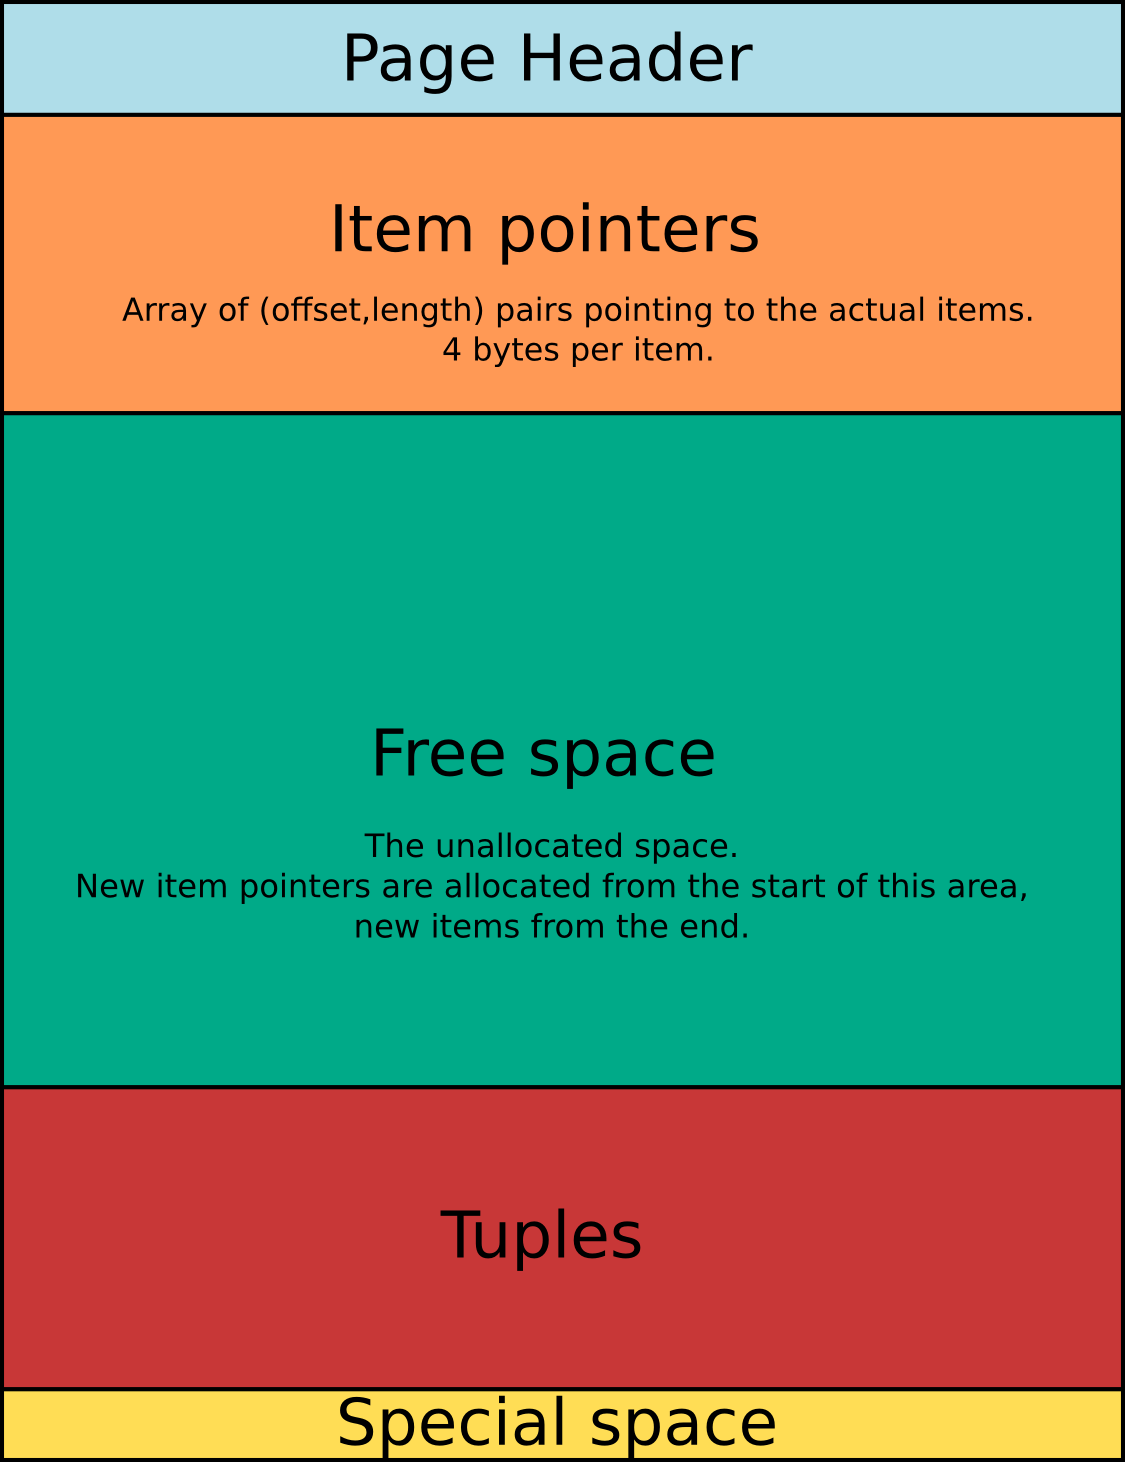
\includegraphics[scale=0.35]{images/index_page_01.png}

\caption{Index page}
\label{fig:INDEX01} 
\end{center}

\end{figure}

A data page starts with a header of \index{Data pages,header}24 bytes. After the 
header there are the item pointers, which size is usually 4 bytes. Each item 
pointer\index{Item pointers} is an array of pairs composed by the offset and the length 
of the item which ponints the physical tuples in the page's bottom.\newline 

The page header holds the information for the page's generic space management as shown 
in figure \ref{fig:HEADERPAG01}. 


\begin{figure}[H]
\begin{center}

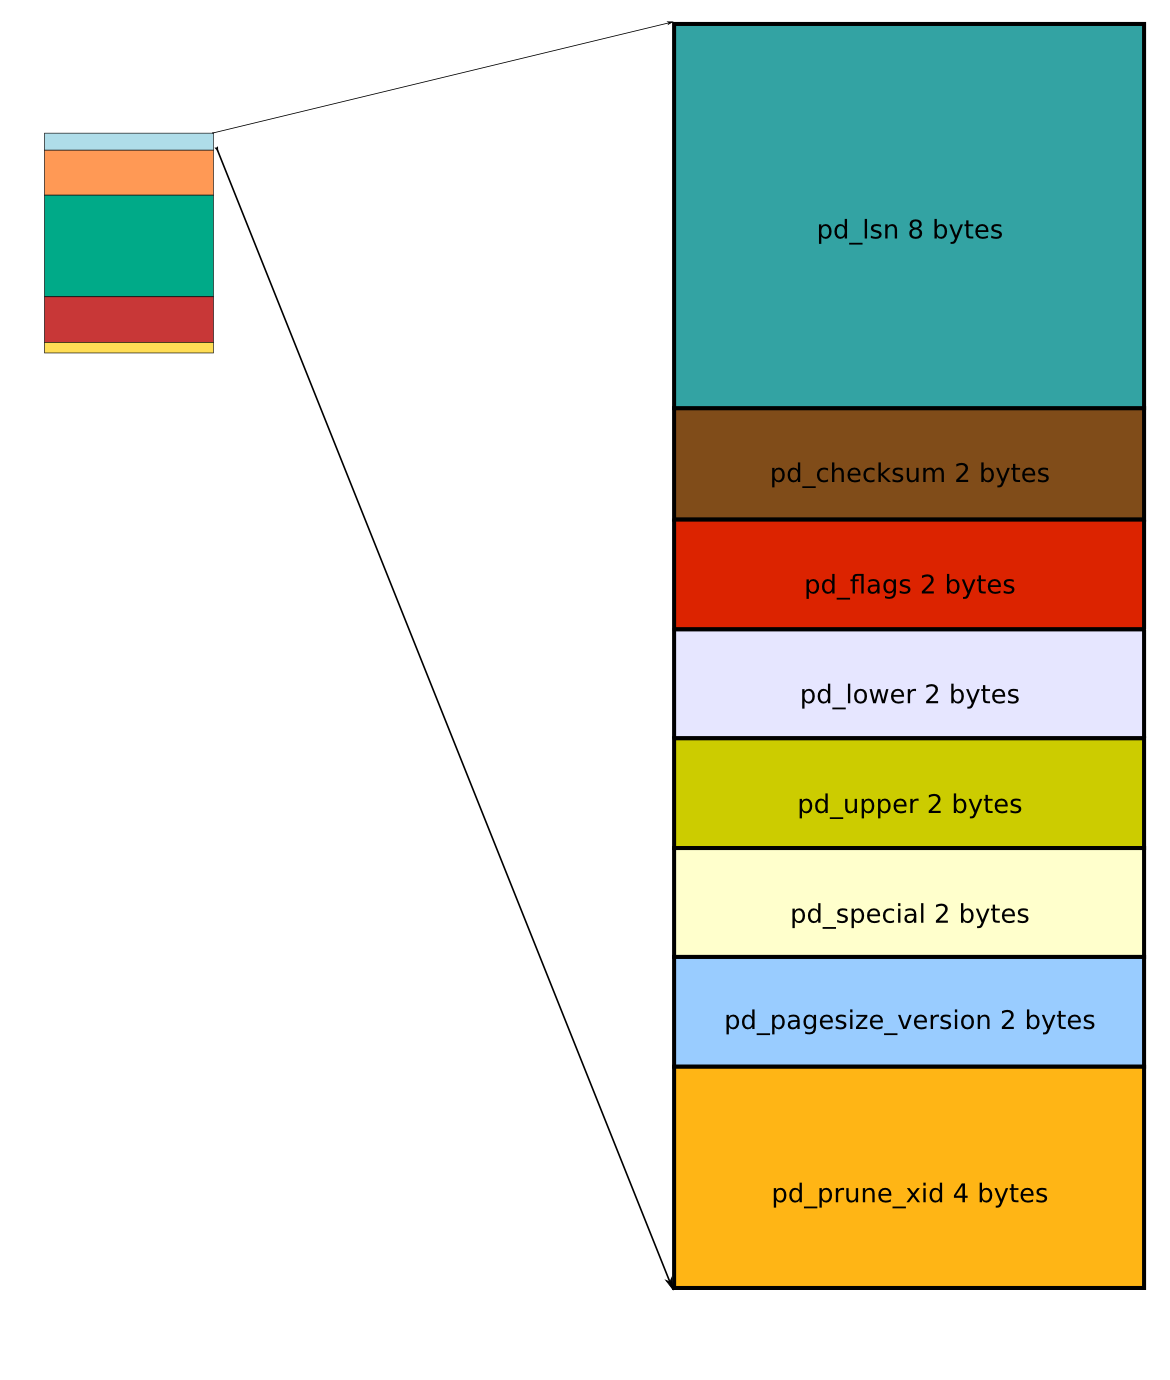
\includegraphics[scale=0.55]{images/header_page_01.png}

\caption{Page header}
\label{fig:HEADERPAG01} 
\end{center}

\end{figure}
\begin{itemize}
 \item \textbf{pd\_lsn} identifies the xlog record for last page's change.  The 
buffer manager uses the  LSN for enforcing the WAL mechanism. A dirty buffer is not 
dumped to the disk until the xlog has been flushed at least as far as the page's LSN.
\item \textbf{pd\_checksum} stores the page's checksum if is enabled.
\item \textbf{pd\_flags} is used to store the page's various flags 
\item \textbf{pg\_lower} is the offset to the start of the free space
\item \textbf{pg\_upper} is the offset to the end of the free space
\item \textbf{pg\_special} is the offset to the start of the special space
\item \textbf{pd\_pagesize\_version} is the page size and the page version packed 
together in a single field. 
\item \textbf{pg\_prune\_xid} is a hint field to determine if the tuple's pruning is 
useful. Is set only on the heap pages.

\end{itemize}

The pd\_checksum \index{Page checksum}field replaces the pd\_tli field present in the page 
header until PostgreSQL 9.2 which was used to track the xlog records across the timeline id. 
\newline 

The page's checksum is a new 9.3's feature which can detects the page corruption. It can be enabled only 
when the data area is initialised with initdb.\newline

The offset fields, pg\_lower, pd\_upper and the optional pd\_special, are 2 bytes long limiting the 
max page size to 32KB.\newline

The field for the page version\index{Page version} was introduced with PostgreSQL 7.3. 
Table \ref{tab:PGPAGEVERSION} shows the page version number for the major versions.

\begin{table}[h]
  \begin{tabular}{cc}
    PostgreSQL version & Page version\\
    \hline
    \textgreater \space 8.3  &  4\\
    8.1,8.2  &  3\\
    8.0  &  2\\
    7.4,7.3  &  1\\
    \textless \space 7.3  &  0\\
    
    
  \end{tabular}
  \caption{\label{tab:PGPAGEVERSION}PostgreSQL page version}
\end{table}

\section{Tuples}\index{Tuples}
\label{sec:TUPLES}
The tuples are the fundamental storage unit in PostgreSQL. They are organised as array of items which kind 
is initially unknown, the datum. Each tuple have a fixed header of 23 bytes as shown in the figure 
\ref{fig:TUPLES01}.\newline

\begin{figure}[H]
\begin{center}

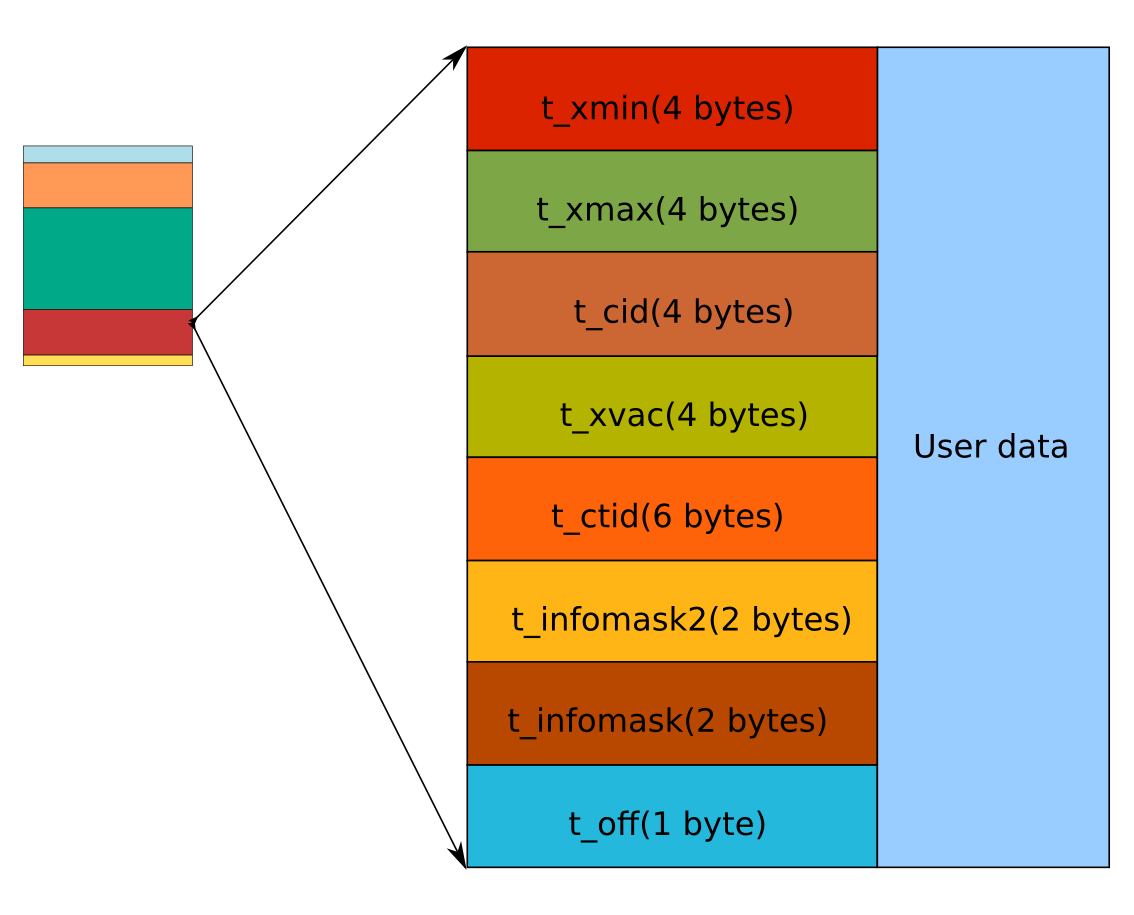
\includegraphics[scale=0.55]{images/tuples_01.png}

\caption{Tuple structure}
\label{fig:TUPLES01} 
\end{center}

\end{figure}

The fields t\_xmin\index{t\_xmin} and t\_xmax\index{t\_xmax} are used to track the tuple's visibility as 
seen in \ref{sec:MVCC}. The field t\_cid\index{t\_cid} is a ``virtual'' field and is used either for cmin 
and cmax. \newline

The field t\_xvac\index{t\_xvac} is used by VACUUM when moving the rows, according with the source code's 
comments in src/include/access/htup\_details.h this field is used only by the old style VACUUM FULL. 
\newline

The field t\_cid\index{t\_cid} is the tuple's physical location identifier. Is composed by a couple of 
integers representing the page number and the tuple's index along the page. When a new tuple is created 
t\_cid is set to the actual row's value. When the tuple is updated the this 
value changes to the new tuple's version location. This field is used in pair with t\_xmax to check if 
the tuple is the last version. The two infomask fields are used to store various flags like the presence of 
the tuple's OID or if the tuple have NULL values. The last field t\_off is used to set the offset to the 
actual tuple's data. This field's value is usually zero if the table doesn't have NULLable fields or is 
created WITHOUT OIDS. If the tuples have the OID and or a NULLable fields, the object identifier and 
a NULL bitmap are stored immediately after the tuple's header. The bitmap if present begins just after the 
tuple's header and consumes enough bytes to have one bit per data column. The OID if present is stored 
after the bitmap and consumes 4 bytes. The tuple's data is a stream of composite data described by the 
composite model stored in the system catalogue. 


\section{TOAST}\index{TOAST}
\label{sec:TOAST}
The oversize attribute storage technique is the PostgreSQL implementation for storing the data 
which overflows the page size. PostgreSQL does not allow the tuples spanning multiple pages. However is 
possible to store large amount of data which is compressed or split in multiple rows in an external 
TOAST table. The mechanism is completely transparent from the user's point of view.\newline

The storage model treats the fixed length, like the integers, and the variable length types, like text, in 
a different way. The fixed length types which cannot produce large data are not processed through the TOAST 
routines. The variable length types are TOASTable if the first 32-bit word of any stored value contains the 
total length of the value in bytes (including itself).

The kind of the TOAST is stored in the first two bits\footnote{On the big-endian architecture those are the 
high-order bits; on the little-endian those are the low-order bits} of the varlena\index{varlena} length 
word. When both bits are zero then the attribute is an unTOASTed data type. In the remaining bits is stored 
the datum size in bytes including the length word.\newline

If the first bit is set then the value have only a single-byte header instead of the four byte header. 
In the remaining bits is stored the total datum size in bytes including the length byte. This scenario 
have a special case uf the remaining bits are all zero. This means the value is a pointer to an out of line 
data stored in a separate TOAST table which structure is shown in figure \ref{fig:TOAST01}.\newline

Finally, whether is the first bit,  if the second bit is set then the corresponding datum is compressed and 
must be decompressed before the use.\newline

Because the TOAST usurps the first two bits of the varlena length word it limits the max stored size to 1 
GB  \begin{math} (2^{30} -1 bytes) \end{math} .

\begin{figure}[H]
\begin{center}

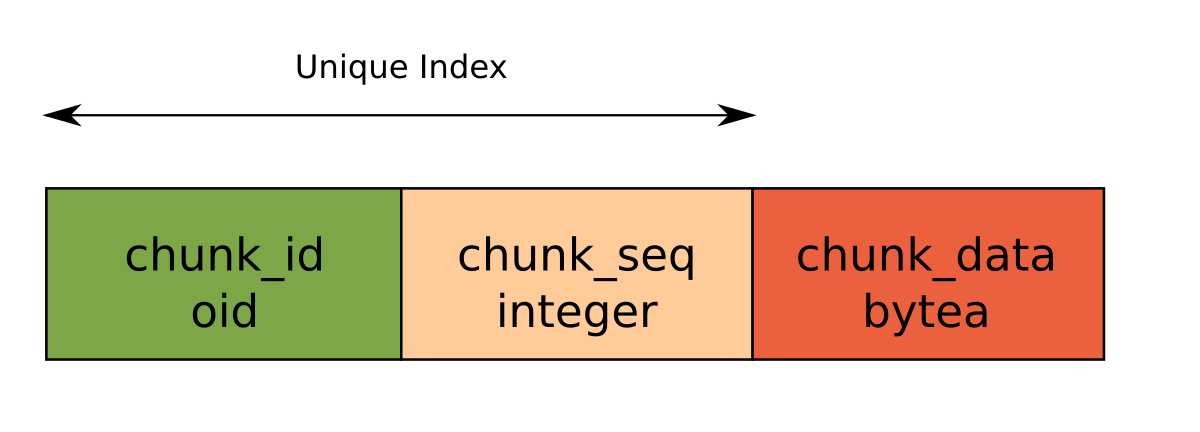
\includegraphics[scale=0.55]{images/toast_01.png}

\caption{Toast table structure}
\label{fig:TOAST01} 
\end{center}

\end{figure}

The toast table is composed by three fields. The chunk\_id is an OID used to store the chunk identifiers. 
The chunk\_seq is an integer which stores the chunk orders. The chunk\_data is a bytea field containing the 
the actual data converted in a binary string.\newline 

The chunk size is normally 2k and is controlled at compile time by the symbol\newline 
TOAST\_MAX\_CHUNK\_SIZE. The TOAST code is triggered by the value\newline  TOAST\_TUPLE\_THRESHOLD, also 2k 
by default. When the tuple's size is 
bigger than \newline TOAST\_TUPLE\_THRESHOLD then the TOAST routines are triggered.\newline

The TOAST\_TUPLE\_TARGET, default 2 kB, governs the compression's behaviour. PostgreSQL will compress the 
datum to achieve a final size lesser than \newline TOAST\_TUPLE\_TARGET. Otherwise the out of line storage 
is used.

TOAST offers four different storage strategies. Each strategy can be changed per column using the  ALTER 
TABLE SET STORAGE statement.
\begin{itemize}

\index{TOAST, storage strategies}
\item  PLAIN prevents either compression or out-of-line storage; It's the only storage available 
for fixed length data types.

\item  EXTENDED allows both compression and out-of-line storage. It is the default for most 
TOAST-able data types. Compression will be attempted first, then out-of-line storage if the row is 
still too big.

\item  EXTERNAL allows out-of-line storage but not compression. 

\item  MAIN allows compression but not out-of-line storage. Actually the out-of-line storage is 
still performed as last resort.

\end{itemize}

The out of line storage\index{TOAST, out of line storage} have the advantage of leaving out the 
stored data from the row versioning; if the TOAST data is not affected by the update there will be 
no dead row for the TOAST data. That's possible because the varlena is a mere pointer to the chunks 
and a new row version will affect only the pointer leaving the TOAST data unchanged.\newline
The TOAST table are stored like all the other relation's in the pg\_class table, the associated 
table can be found using a self join on the field reltoastrelid.\newline


\section{Tablespaces}\index{tablespaces,physical}
\label{sub:TBS-PHYSICAL}
PostgreSQL implements the tablespaces with the symbolic links. Inside the directory \$PGDATA/pg\_tblspc 
there are the links to the physical location. Each link is named after the tablespace's OID. Therefore the 
tablespaces are available only on the systems with the symbolic link support.\newline

Before the version 8.4 the tablespace symbolic link pointed directly to the referenced directory. This was 
a race condition when upgrading in place because the the location could clash with the upgraded cluster. 
From the version 9.0, the tablespace creates a sub directory directory in the tablespace location which 
is after the major version and the system catalogue version number. 
\newline

\begin{verbatim}

postgres@tardis:~$ ls -l /var/lib/postgresql/pg_tbs/ts_test
total 0
drwx------ 2 postgres postgres 6 Jun  9 13:01 PG_9.3_201306121

\end{verbatim}

The sub directory's name is a combination of the capital letters PG followed by the major version, 
truncated to the first two numbers, and the catalogue version number stored in the control file.\newline



\begin{verbatim}
postgres@tardis:~$ export PGDATA=/var/lib/postgresql/9.3/main
postgres@tardis:~$ /usr/lib/postgresql/9.3/bin/pg_controldata 
pg_control version number:            937
Catalog version number:               201306121
Database system identifier:           5992975355079285751
Database cluster state:               in production
pg_control last modified:             Mon 09 Jun 2014 13:05:14 UTC
.
.
.
WAL block size:                       8192
Bytes per WAL segment:                16777216
Maximum length of identifiers:        64
Maximum columns in an index:          32
Maximum size of a TOAST chunk:        1996
Date/time type storage:               64-bit integers
Float4 argument passing:              by value
Float8 argument passing:              by value
Data page checksum version:           0



PG_{MAJOR_VERSION\}_{CATALOGUE_VERSION_NUMBER}

\end{verbatim}



Inside the container directory the data files are organised in the same way as in base directory.
\ref{sec:PGDATA}.\newline

Moving a tablespace to another physical location it's not complicated but the cluster needs to be shut down.
With the cluster stopped the container directory can be safely copied to the new location. The receiving 
directory must have the same permissions  like the origin's. The symbolic link must be recreated to point 
to the new physical location. At the cluster's start the change will be automatically resolved from 
the symbolic link.\newline

Until PostgreSQL 9.1 the tablespace location was stored into the field spclocation in the system table 
pg\_tablespace\index{pg\_tablespace}. From the version 9.2 the spclocation field is removed and the 
tablespace's location is resolved on the fly using the function 
pg\_tablespace\_location(tablespace\_oid).\newline

This function can be used to query the system catalogue about the tablespaces. In this simple example the 
query returns the tablespace's location resolved from the OID. 

\begin{lstlisting}[style=pgsql]
postgres=# 
                SELECT 
                        pg_tablespace_location(oid),
                        spcname 
                FROM 
                        pg_tablespace
                ;
        
       pg_tablespace_location       |  spcname   
------------------------------------+------------
                                    | pg_default
                                    | pg_global
 /var/lib/postgresql/pg_tbs/ts_test | ts_test
(3 rows)

\end{lstlisting}

Because the function pg\_tablespace\_location returns the empty string for the system tablespaces, a better 
approach is combining the CASE construct with the function current\_settings and build the absolute path 
for the system tablespaces.

\begin{lstlisting}[style=pgsql]
 postgres=# SELECT current_setting('data_directory');
       current_setting        
------------------------------
 /var/lib/postgresql/9.3/main
(1 row)

postgres=# 
SELECT 
        CASE
                WHEN 
                                pg_tablespace_location(oid)=''
                        AND     spcname='pg_default'
                THEN
                        current_setting('data_directory')||'/base/'
                WHEN 
                                pg_tablespace_location(oid)=''
                        AND     spcname='pg_global'
                THEN
                        current_setting('data_directory')||'/global/'
        ELSE
                pg_tablespace_location(oid)
        END
        AS      spclocation,
                
        spcname 
FROM 
        pg_tablespace;
             spclocation              |  spcname   
--------------------------------------+------------
 /var/lib/postgresql/9.3/main/base/   | pg_default
 /var/lib/postgresql/9.3/main/global/ | pg_global
 /var/lib/postgresql/pg_tbs/ts_test   | ts_test
(3 rows)

\end{lstlisting}

Another useful function the pg\_tablespace\_databases(tablespace\_oid) can help us to find the databases 
with the relations on a certain tablespace.\newline

The following example uses this function again with a CASE construct for building the database having 
objects on a specific tablespace, in our example the ts\_test created in \ref{sub:TBS-LOGICAL}.\newpage
\begin{lstlisting}[style=pgsql]
 db_test=# 
 SELECT
        datname,
        spcname,
        CASE
                WHEN 
                                pg_tablespace_location(tbsoid)=''
                        AND     spcname='pg_default'
                THEN
                        current_setting('data_directory')||'/base/'
                WHEN 
                                pg_tablespace_location(tbsoid)=''
                        AND     spcname='pg_global'
                THEN
                        current_setting('data_directory')||'/global/'
        ELSE
                pg_tablespace_location(tbsoid)
        END
        AS      spclocation
FROM
        pg_database dat,
        (
                SELECT
                        oid as tbsoid,
                        pg_tablespace_databases(oid) as datoid,
                        spcname 
                FROM 
                        pg_tablespace where spcname='ts_test'
        ) tbs
WHERE
        dat.oid=tbs.datoid
;
 datname | spcname |            spclocation             
---------+---------+------------------------------------
 db_test | ts_test | /var/lib/postgresql/pg_tbs/ts_test
(1 row)

\end{lstlisting}



\section{MVCC} \label{sec:MVCC}\index{MVCC} 
The multiversion concurrency control is used in PostgreSQL to implement the  transactional model seen in 
\ref{sec:TRANSACTION}.\newline

At logical level this is completely transparent to the user and the new row versions become visible 
after the commit, accordingly with the transaction isolation level. \newline

At physical level we have for each new row version, the insert's XID stored into the t\_xmin field which is 
used by the internal semantic to determine the row visibility. 

Because the XID is a 32 bit quantity, it wraps at 4 billions. When this happens theoretically all 
the tuples should suddenly disappear because they switch from in the current XID's past to its future in 
the well known XID wraparound failure,\index{XID wraparound failure}. In the old PostgreSQL versions this 
was a serious problem which forced the administrators to dump/reload the entire cluster into a freshly 
initialised new data area every 4 billion of transactions.\newline 

In PostgreSQL 7.2 was introduced a new comparison method for the XID, the 
\begin{math}modulo-2^{32}\end{math} arithmetic. It was also introduced a special XID, the 
FrozenXID\footnote{The FrozenXID's value is 2. The docs of PostgreSQL 
7.2 also mention the BootstrapXID which value is 1} assumed as always in the past. With the new 
comparison method, for any arbitrary XID exists 2 billion of transactions in the future and 2 billion 
transactions in the past.\newline

When the age of the tuple's t\_xmin becomes old the periodic VACUUM\index{VACUUM} freezes the ageing tuple 
changing its t\_xmin to the FrozenXID always in the past. In the pg\_class and the pg\_database tables 
there are  two dedicated fields to track the age of the oldest XID. The value stored in those tables 
have little meaning if not processed through the function age() which shows the number of transactions 
between the current XID and the value stored in the system catalogue. \newline

This following query returns all the databases, the corresponding datfrozenxid and the XID's age.\newpage

\begin{lstlisting}[style=pgsql]
 postgres=# 
        SELECT 
                datname,
                age(datfrozenxid),
                datfrozenxid 
        FROM 
                pg_database;
    datname    | age  | datfrozenxid 
---------------+------+--------------
 template1     | 4211 |          679
 template0     | 4211 |          679
 postgres      | 4211 |          679
 db_test       | 4211 |          679

\end{lstlisting}

When a tuple's age is more than 2 billions the tuple simply disappears  from the cluster. Before the 
version 8.0 there was no alert or protection against the XID wraparound failure. Since then it was 
introduced a passive mechanism which emits messages in the activity log when the age of datfrozenxid 
is less than ten million transactions from the wraparound point.

A message like this is quite serious and should not be ignored.
\begin{smallverbatim}
WARNING:  database "test_db" must be vacuumed within 152405486 transactions
HINT:  To avoid a database shutdown, execute a database-wide VACUUM in 
"test_db".
\end{smallverbatim}

The autovacuum daemon in this case acts like a watchdog and starts vacuuming the tables with ageing 
tuples even  if autovacuum is turned off in the cluster. There is another protection, quite radical, 
if for some reasons one of the database's datfrozenxid is at one million transactions from the 
wraparound point. In this case the cluster shuts down and refuse to start again. The only option in 
this case is to run the postgres process in single-user backend and execute the VACUUM on the 
affected relations.\newline

The debian package's configuration is quite odd, putting the configuration files in the /etc/postgresql 
instead of the data area. The following example is the standalone backend's call for the debian's packaged 
default cluster main.

\begin{verbatim}

postgres@tardis:~/tempdata$ /usr/lib/postgresql/9.3/bin/postgres \
--single -D /var/lib/postgresql/9.3/main/base/ \
--config-file=/etc/postgresql/9.3/main/postgresql.conf

PostgreSQL stand-alone backend 9.3.5
backend> 

\end{verbatim}

The database interface in single user mode and does not have all the sophisticated features 
like the client psql. Anyway with a little knowledge of SQL it's possible to find the database(s) 
causing the shutdown and fix it.
\index{postgres, single user mode}\index{XID wraparound failure, fix}

\begin{verbatim}
backend> SELECT datname,age(datfrozenxid) FROM pg_database ORDER BY 2 DESC;

1: datname     (typeid = 19, len = 64, typmod = -1, byval = f)
2: age (typeid = 23, len = 4, typmod = -1, byval = t)
----
1: datname = "template1" (typeid = 19, len = 64, typmod = -1, byval = f)
2: age = "2146435072"  (typeid = 23, len = 4, typmod = -1, byval = t)
----
1: datname = "template0" (typeid = 19, len = 64, typmod = -1, byval = f)
2: age = "10"  (typeid = 23, len = 4, typmod = -1, byval = t)
----
1: datname = "postgres"  (typeid = 19, len = 64, typmod = -1, byval = f)
2: age = "10"  (typeid = 23, len = 4, typmod = -1, byval = t)
----

\end{verbatim}

The age function shows how old is the last XID not yet frozen. In our example the template1
database have an age of 2146435072, one million transactions to the wraparound. We can then exit 
the backend with CTRL+D and restart it again in the in single user mode specifying the database 
name. A VACUUM will get rid of the problematic xid.

\begin{verbatim}
postgres@tardis:~/tempdata$ /usr/lib/postgresql/9.3/bin/postgres \
--single -D /var/lib/postgresql/9.3/main/base/ \
--config-file=/etc/postgresql/9.3/main/postgresql.conf \
template1
                                
backend> SELECT current_database();
1: current_database (typeid = 19, len = 64, typmod = -1, byval = f)
----
1: current_database = "template1" (typeid = 19, len = 64, typmod = -1, byval = f)
----

backend> VACUUM FREEZE;
\end{verbatim}

This procedure must be repeated for any database with very old XID.\newline

Because the new rows generation at update time, this can lead to an unnecessary table and index bloat.
PostgreSQL with the Heap Only Tuples (HOT)\index{HOT strategy} strategy can limit the unavoidable bloat 
caused by the updates. HOT's main goal is to keep the new row versions into the same page. 

The MVCC is something to consider at design time. Ignoring the way PostgreSQL manages the physical tuples 
can result in data bloat and lead in general to poor performances.

\chapter{Maintenance}
\label{cha:MAINTENANCE}\index{Maintenance}
The database maintenance is something crucial for keeping the data access efficient. Building a proper 
maintenance plan is almost important like having a good disaster recovery plan.\newline

As seen in \ref{sec:MVCC} the update generates new tuple's version rather updating the affected field. 
The new tuple is stored in the next available free space in the same page or a different one. 
Frequent updates will in move the tuples across the data pages many and many times with a trail of dead 
tuples. Unfortunately those tuples although consuming physically space, are no longer visible for the 
new transactions and this results in the table bloat. The indices make things more complicated. When a new 
tuple's version is stored in a different page the index entry needs update to point the new page. The the 
index's ordered structure makes more difficult to find free space, resulting in an higher rate of new 
pages added to the relation and consequent bloat. \newline

The following sections will explore the tools available for the relation's maintenance.

\section{VACUUM}\index{VACUUM}
\label{sec:VACUUM}
VACUUM is a PostgreSQL specific command which reclaims back the dead tuple's space. When executed without a 
target table, the command scans all the tables in the database. A regular VACUUM have some beneficial 
effects.

\begin{itemize}
 \item Removes the dead tuples and updates the free space map.
 \item Updates the visibility map improving the index only scans.
 \item It freezes the tuples with ageing XID preventing the XID wraparound\index{XID wraparound 
failure} 
\end{itemize}

The optional ANALYZE clause gathers the runtime statistics on processed table.\newline

When run VACUUM clear the space used by the dead rows making space for the inserts and updates inside the 
data files. The data files are not shrunk except if there is a contiguous free space in the table's 
end. VACUUM in this case runs a truncate scan which can fail if there is a conflicting lock with the 
database activity. The VACUUM's truncate scan works only on the table's data files. The general approach 
for VACUUM is to have the minimum the impact on the cluster's activity. However, because the pages are 
rewritten, VACUUM can increase the I/O activity.\newline

The index pages are scanned as well and the dead tuples are also cleared. The VACUUM performances on the 
indices are influenced by the maintenance\_work\_mem setting. If the table does not have indices VACUUM 
will run the cleanup reading the pages sequentially. If there is any index VACUUM will store in the 
maintenance work memory  the tuple's references for the subsequent index cleanup. If the memory is 
not sufficient to fit all the tuples then VACUUM will stop the sequential read to execute the 
partial cleanup on the indices and free the maintenance worm mem.\newline

The the maintenance\_work\_mem  can impact sensibly on the VACUUM's performance on large tables. For example 
let's build build a simple table with 10 million rows. 


\begin{lstlisting}[style=pgsql]
postgres=# CREATE TABLE t_vacuum 
        (
                i_id serial,
                t_ts_value timestamp with time zone DEFAULT clock_timestamp(),
                t_value text,
                CONSTRAINT pk_t_vacuum PRIMARY KEY  (i_id)
        )
;

CREATE TABLE

postgres=# INSERT INTO t_vacuum
        (t_value)
SELECT 
         md5(i_cnt::text)
FROM
(
        SELECT
                generate_series(1,10000000) as i_cnt
) t_cnt
;
INSERT 0 10000000


\end{lstlisting}
In order to have a static environment we'll disable the table's autovacuum. We'll also increase the 
session's verbosity display what's happening during the VACUUM's run.\newline

\begin{lstlisting}[style=pgsql]
postgres=# ALTER TABLE t_vacuum 
        SET 
                (
                        autovacuum_enabled = false, 
                        toast.autovacuum_enabled = false
                )
;
ALTER TABLE


SET client_min_messages='debug';

\end{lstlisting}

We are now executing a complete table rewrite running an UPDATE without the WHERE condition. 
This will create 10 millions of dead rows.\newline

\begin{lstlisting}[style=pgsql]
postgres=# UPDATE t_vacuum 
        SET 
                t_value = md5(clock_timestamp()::text)
;
UPDATE 10000000

\end{lstlisting}

Before running the VACUUM we'll change the maintenance\_work\_mem to a small value. We'll also enable the 
query timing.\newline

\begin{lstlisting}[style=pgsql]
postgres=# SET maintenance_work_mem ='20MB';
SET
postgres=# \timing
Timing is on.

postgres=# VACUUM t_vacuum;
DEBUG:  vacuuming "public.t_vacuum"
DEBUG:  scanned index "pk_t_vacuum" to remove 3495007 row versions
DETAIL:  CPU 0.80s/4.56u sec elapsed 21.36 sec.
DEBUG:  "t_vacuum": removed 3495007 row versions in 36031 pages
DETAIL:  CPU 0.63s/0.56u sec elapsed 19.31 sec.
DEBUG:  scanned index "pk_t_vacuum" to remove 3495007 row versions
DETAIL:  CPU 0.67s/4.18u sec elapsed 15.28 sec.
DEBUG:  "t_vacuum": removed 3495007 row versions in 36031 pages
DETAIL:  CPU 0.67s/0.53u sec elapsed 18.07 sec.
DEBUG:  scanned index "pk_t_vacuum" to remove 3009986 row versions
DETAIL:  CPU 0.53s/2.86u sec elapsed 12.29 sec.
DEBUG:  "t_vacuum": removed 3009986 row versions in 31031 pages
DETAIL:  CPU 0.47s/0.52u sec elapsed 20.06 sec.
DEBUG:  index "pk_t_vacuum" now contains 10000000 row versions in 82352 pages
DETAIL:  10000000 index row versions were removed.
0 index pages have been deleted, 0 are currently reusable.
CPU 0.00s/0.00u sec elapsed 0.00 sec.
DEBUG:  "t_vacuum": found 10000000 removable, 10000000 nonremovable row versions in 206186 out of 
206186 pages
DETAIL:  0 dead row versions cannot be removed yet.
There were 0 unused item pointers.
0 pages are entirely empty.
CPU 5.92s/17.08u sec elapsed 154.10 sec.
DEBUG:  vacuuming "pg_toast.pg_toast_28499"
DEBUG:  index "pg_toast_28499_index" now contains 0 row versions in 1 pages
DETAIL:  0 index row versions were removed.
0 index pages have been deleted, 0 are currently reusable.
CPU 0.00s/0.00u sec elapsed 0.00 sec.
DEBUG:  "pg_toast_28499": found 0 removable, 0 nonremovable row versions in 0 out of 0 pages
DETAIL:  0 dead row versions cannot be removed yet.
There were 0 unused item pointers.
0 pages are entirely empty.
CPU 0.00s/0.00u sec elapsed 0.00 sec.
VACUUM
Time: 154143.383 ms
postgres=# 


\end{lstlisting}

VACUUM stores in the maintenance\_work\_mem an array of TCID pointers to the removed dead tuples. This 
is used for the index cleanup. With a small maintenance\_work\_mem the array can consume the entire 
memory causing VACUUM to pause the table scan for a partial index cleanup. The table scan then resumes. 
Increasing the maintenance\_work\_mem to 2 GB\footnote{In order to have the table in the same conditions the 
table was cleared with a VACUUM FULL and bloated with a new update.} the index scan without pauses 
which improves the VACUUM's speed.\newline

\begin{lstlisting}[style=pgsql]
postgres=# SET maintenance_work_mem ='2GB';
SET

postgres=# VACUUM t_vacuum;
DEBUG:  vacuuming "public.t_vacuum"
DEBUG:  scanned index "pk_t_vacuum" to remove 10000000 row versions
DETAIL:  CPU 1.58s/8.45u sec elapsed 52.41 sec.
DEBUG:  "t_vacuum": removed 10000000 row versions in 103093 pages
DETAIL:  CPU 1.78s/1.41u sec elapsed 33.90 sec.
DEBUG:  index "pk_t_vacuum" now contains 10000000 row versions in 82352 pages
DETAIL:  10000000 index row versions were removed.
0 index pages have been deleted, 0 are currently reusable.
CPU 0.00s/0.00u sec elapsed 0.00 sec.
DEBUG:  "t_vacuum": found 10000000 removable, 10000000 nonremovable row versions in 206186 out of 
206186 pages
DETAIL:  0 dead row versions cannot be removed yet.
There were 0 unused item pointers.
0 pages are entirely empty.
CPU 5.62s/13.64u sec elapsed 121.99 sec.
DEBUG:  vacuuming "pg_toast.pg_toast_28499"
DEBUG:  index "pg_toast_28499_index" now contains 0 row versions in 1 pages
DETAIL:  0 index row versions were removed.
0 index pages have been deleted, 0 are currently reusable.
CPU 0.00s/0.00u sec elapsed 0.00 sec.
DEBUG:  "pg_toast_28499": found 0 removable, 0 nonremovable row versions in 0 out of 0 pages
DETAIL:  0 dead row versions cannot be removed yet.
There were 0 unused item pointers.
0 pages are entirely empty.
CPU 0.00s/0.00u sec elapsed 0.00 sec.
VACUUM
Time: 122021.251 ms


\end{lstlisting}

Without the indices VACUUM completes in the shortest time.\newline

\begin{lstlisting}[style=pgsql]

postgres=# SET maintenance_work_mem ='20MB';
SET
postgres=# \timing
Timing is on.

postgres=# ALTER TABLE t_vacuum DROP CONSTRAINT pk_t_vacuum;
DEBUG:  drop auto-cascades to index pk_t_vacuum
ALTER TABLE
Time: 182.737 ms

postgres=# VACUUM t_vacuum;
DEBUG:  vacuuming "public.t_vacuum"
DEBUG:  "t_vacuum": removed 10000000 row versions in 103093 pages
DEBUG:  "t_vacuum": found 10000000 removable, 10000000 nonremovable row versions in 206186 out of 
206186 pages
DETAIL:  0 dead row versions cannot be removed yet.
There were 0 unused item pointers.
0 pages are entirely empty.
CPU 2.16s/4.53u sec elapsed 47.30 sec.
DEBUG:  vacuuming "pg_toast.pg_toast_28499"
DEBUG:  index "pg_toast_28499_index" now contains 0 row versions in 1 pages
DETAIL:  0 index row versions were removed.
0 index pages have been deleted, 0 are currently reusable.
CPU 0.00s/0.00u sec elapsed 0.00 sec.
DEBUG:  "pg_toast_28499": found 0 removable, 0 nonremovable row versions in 0 out of 0 pages
DETAIL:  0 dead row versions cannot be removed yet.
There were 0 unused item pointers.
0 pages are entirely empty.
CPU 0.00s/0.00u sec elapsed 0.00 sec.
VACUUM
Time: 48823.132 ms




\end{lstlisting}

The table seen in the example begins with a size of 806 MB . After the update the table's size is doubled. 
After the VACUUM run the table does not shrink. This is caused because there is no contiguous free space in 
the end. The new row versions generated by the update are stored in the table's end. A second UPDATE 
with a new VACUUM could truncate the table if all the dead rows are in the table's end. However 
VACUUM's main goal is to keep the table's size stable, rather shrinking down the space.\newline

The prevention of the XID wraparound failure managed automatically by VACUUM. When a live tuple have the 
t\_xmin's older than the parameter vacuum\_freeze\_min\_age, then the t\_xid replaced with the 
FrozenXID setting the tuple safely in the past. Because VACUUM by default skips the pages without dead 
tuples some ageing tuples could be skipped by the run. The parameter vacuum\_freeze\_table\_age avoids 
this scenario triggering a full table's VACUUM when table's relfrozenxid age exceeds the value.\newline

It's also possible to run VACUUM with the FREEZE \index{VACUUM FREEZE} clause. In this case VACUUM 
will freeze all the tuples regardless of their age. The command is equivalent of running VACUUM with 
vacuum\_freeze\_min\_age set to zero.\newline

VACUUM is controlled by some GUC parameters.

\subsection{vacuum\_freeze\_table\_age}
This parameter is used to start a full table VACUUM when the table's relfrozenxid exceeds the parameter's 
value. The default setting is 150 million of transactions. Despite the possible values are between zero 
and one billion, VACUUM will silently set the effective value to the 95\% of 
the autovacuum\_freeze\_max\_age, reducing the possibility to have an anti-wraparound autovacuum.

\subsection{vacuum\_freeze\_min\_age}
The parameter sets minimum age for the tuple's t\_xmin to be frozen. The default is 50 million 
transactions. The values accepted are between zero to one billion. However VACUUM will change silently the 
effective value to one half of autovacuum\_freeze\_max\_age in order to maximise the time between the 
forced autovacuum.

\subsection{vacuum\_multixact\_freeze\_table\_age}
From PostgreSQL 9.3 VACUUM maintains the multixact ID as well. This identifier is used to store the 
row locks in the tuple's header.  Because the multixact ID\index{multixact ID} is a 32 bit quantity there 
is the same XID's issue with the wraparound failure\index{multixact ID, wraparound failure}. This parameter 
sets the value after that a table scan is performed. The setting is checked against the field relminmxid of 
the pg\_class. The default is 150 million of multixacts. The accepted values are between zero and one 
billion. VACUUM limits the effective value to the 95\% of autovacuum\_multixact\_freeze\_max\_age. This wat 
the manual VACUUM has a chance to run before an anti-wraparound autovacuum.

\subsection{vacuum\_multixact\_freeze\_min\_age}
Sets the minimum age in multixacts for VACUUM to replace the multixact IDs with a newer transaction ID or 
multixact ID, while scanning a table. The default is 5 million multixacts. The accepted values 
are between zero and one billion. VACUUM will silently limit the effective value to one half of 
autovacuum\_multixact\_freeze\_max\_age, in order to increase the time between the forced autovacuums.

\subsection{vacuum\_defer\_cleanup\_age}
This parameter have effect only on the master in the hot standby configurations. When set to a positive  
value on the master, can reduce the risk of query conflicts on the standby. Does not have effect on a 
standby server.

\subsection{vacuum\_cost\_delay}\label{sub:VACUUMCOST}
This parameter, if set to a not zero value enables the cost based vacuum delay\index{VACUUM, cost 
based delay} and sets the sleep time, in milliseconds, for VACUUM process when the cost limit exceeds. The 
default value is zero, which disables the cost-based vacuum delay feature. 

\subsection{vacuum\_cost\_limit}
This parameter sets the arbitrary cost limit. VACUUM sleeps for the time set in vacuum\_cost\_delay when 
the value is reached. The default value is 200. 

\subsection{vacuum\_cost\_page\_hit}
The parameter sets the arbitrary cost for vacuuming one buffer found in the shared buffer cache. It 
represents the cost to lock the buffer, look up to the shared hash table and scan the content of the page. 
The default value is one.

\subsection{vacuum\_cost\_page\_miss}
This parameter sets the arbitrary cost for vacuuming a buffer not present in the shared buffer. This 
represents the effort to lock the buffer pool, lookup the shared hash table, read the desired block 
from the disk and scan its content. The default value is 10.

\subsection{vacuum\_cost\_page\_dirty}
This parameter sets the arbitrary cost charged when vacuum scans a previously dirty page\footnote{A 
page is dirty when its modifications are not yet written on the relation's data file}. It represents the 
extra I/O required to flush the dirty block out to disk. The default value is 20.

\section{ANALYZE}
\label{sec:ANALYZE}
The PostgreSQL's query optimiser builds the query execution plan using the cost estimates from the 
internal runtime statistics. Each step in the execution plan gets an arbitrary cost used to compute the 
plan total cost. The execution plan which estimated cost is lesser is then sent to the query executor. 
Keeping the runtime statistics up to date helps the cluster to build efficient plans.\newline

The command ANALYZE\index{ANALYZE} gathers the relation's runtime statistics. When executed reads the 
data, builds up the statistics and stores them into the pg\_statistics\index{pg\_statistics, 
table} system table. The command accepts the optional clause VERBOSE to increase verbosity alongside the 
optional target table and the eventual column list. If ANALYZE is launched with no parameters scans all the 
tables in the database. Specifying the table name will cause ANALYZE to process all the table's 
columns.\newline

When working on large tables ANALYZE runs a sample read on the table.  The GUC parameter 
default\_statistics\_target determines the amount of entries read by the sample. The 
default limit is 100. Increasing the value will cause the planner to get better estimates, in particular 
for the columns with the data distributed irregularly. This accuracy have a cost. Will cause ANALYZE to 
spend a longer time for the statistics gathering and building plus an bigger space required 
in pg\_statistics.\newline


The following example will show how default\_statistics\_target can affects the estimates. We'll re use 
the table created in \ref{sec:VACUUM}. This is the result of ANALYZE VERBOSE with the default 
statistic target.

\begin{lstlisting}[style=pgsql]
postgres=# SET default_statistics_target =100;
SET
postgres=# ANALYZE VERBOSE t_vacuum;
INFO:  analyzing "public.t_vacuum"
INFO:  "t_vacuum": scanned 30000 of 103093 pages, containing 2909979 live rows and 0 dead rows; 
30000 rows in sample, 9999985 estimated total rows
ANALYZE
\end{lstlisting}

The table have 10 million rows but ANALYZE estimates the contents in just 2,909,979 rows, the 30\% of 
the effective live tuples.\newline

Now we'll run ANALYZE with default\_statistics\_target set to its maximum allowed value, 10000.


\begin{lstlisting}[style=pgsql]
SET
postgres=# ANALYZE VERBOSE t_vacuum;
INFO:  analyzing "public.t_vacuum"
INFO:  "t_vacuum": scanned 103093 of 103093 pages, containing 10000000 live rows and 0 dead rows; 
3000000 rows in sample, 10000000 estimated total rows
ANALYZE
\end{lstlisting}

This time the table's live tuples are estimated correctly in 10 millions.\newline

The table pg\_statistics is not intended for human reading. The statistics are translated in human 
readable format by the view pg\_stats\index{pg\_stats, view}.\newline

The rule of thumb when dealing with poorly performing queries, is to check if statistics are recent 
and accurate. The information is stored into the view pg\_stat\_all\_tables \footnote{The subset views 
pg\_stat\_user\_tables and pg\_stat\_sys\_tables are useful to search respectively the current user and the 
system tables only.}.

For example this query gets, for a certain table,  the last execution of the manual and the auto vacuum 
alongside with the last analyze and auto analyze.

\begin{lstlisting}[style=pgsql]

postgres=# \x
Expanded display is on.
postgres=# SELECT
        schemaname,
        relname,
        last_vacuum,
        last_autovacuum,
        last_analyze,
        last_autoanalyze
FROM
         pg_stat_all_tables
WHERE
        relname='t_vacuum'
;
-[ RECORD 1 ]----+------------------------------
schemaname       | public
relname          | t_vacuum
last_vacuum      | 
last_autovacuum  | 
last_analyze     | 2014-06-17 18:48:56.359709+00
last_autoanalyze | 

postgres=# 



\end{lstlisting}


The statistics target is a per column setting allowing a fine grained tuning for the ANALYZE command.

\begin{lstlisting}[style=pgsql]


--SET THE STATISTICS TO 1000 ON THE COLUMN i_id
ALTER TABLE t_vacuum 
        ALTER COLUMN  i_id 
                        SET STATISTICS 1000
;

\end{lstlisting}

The default statistic target can be changed for the current session only using the SET command. The cluster 
wide value is changed using the parameter in the postgresql.conf file.

\section{REINDEX}\label{sec:REINDEX}
The general purpose B-tree index stores the indexed value alongside with the pointer to the 
tuple's heap page. The index pages are organised in the form of a balanced tree linking each other 
using page's special space seen in \ref{fig:INDEX01}. As long as the heap tuple remains in the same page
the index entry doesn't need update. The HOT strategy\index{HOT strategy} tries to achieve this goal keeping 
the heap tuples in the same page. When a new tuple version is stored in the heap page then also the index 
entry needs to reflect the change. By default the index pages have a percentage of space reserved for 
the updates. This is an hardcoded 30\% for the not leaf pages and a 10\% for the leaf 
pages. The latter can be changed adjusting the index's fillfactor.\newline

VACUUM efficiency is worse with the indices because their ordered nature. Even converting the dead 
tuples to free space, this is reusable only if the new entry is compatible with the B-tree position. 
The empty pages can be recycled but this requires at least two VACUUM runs. When an index page is empty 
then is marked as deleted by VACUUM but not immediately recycled. The page is first stamped with the next 
XID and therefore becomes invisible. Only a second VACUUM will clear the deleted pages returning the 
free space to the relation. This behaviour is made on purpose, because there might be running 
scans which still need to access the page. The second VACUUM is the safest way to recycle the page only 
if no longer required.\newline

Therefore the indices are affected by the data bloat more than the tables. Alongside with a bigger disk 
space allocation, the bloat results generally in bad index's performances. The periodical reindex 
is the best way to keep the indices in good shape.\newline

Unlike the VACUUM, the REINDEX have a noticeable impact on the cluster's activity. To ensure the data is 
consistently read the REINDEX sets a lock on the table preventing the table's writes. The reads are also 
blocked for the queries which are using the index.\newline

A B-tree index build requires a the data to be sorted. PostgreSQL comes with a handy GUC parameter to track 
the sort, the trace\_sort\index{trace\_sort} which requires a verbosity set to DEBUG.

The following example is the output of the primary key's reindex of the test table created in 
\ref{sec:VACUUM}. 


\begin{lstlisting}[style=pgsql]
postgres=# SET trace_sort =on;
SET
postgres=# SET client_min_messages ='debug';
SET
postgres=# \timing
Timing is on.

postgres=# REINDEX INDEX pk_t_vacuum ;
DEBUG:  building index "pk_t_vacuum" on table "t_vacuum"
LOG:  begin index sort: unique = t, workMem = 16384, randomAccess = f
LOG:  begin index sort: unique = f, workMem = 1024, randomAccess = f
LOG:  switching to external sort with 59 tapes: CPU 0.00s/0.08u sec elapsed 0.08 sec
LOG:  finished writing run 1 to tape 0: CPU 0.13s/3.41u sec elapsed 3.55 sec
LOG:  internal sort ended, 25 KB used: CPU 0.39s/8.35u sec elapsed 8.74 sec
LOG:  performsort starting: CPU 0.39s/8.35u sec elapsed 8.74 sec
LOG:  finished writing final run 2 to tape 1: CPU 0.39s/8.50u sec elapsed 8.89 sec
LOG:  performsort done (except 2-way final merge): CPU 0.40s/8.51u sec elapsed 8.90 sec
LOG:  external sort ended, 24438 disk blocks used: CPU 0.70s/9.67u sec elapsed 11.81 sec
REINDEX
Time: 11876.807 ms

\end{lstlisting}

The reindex performs a data sort which does not fit in the maintenance\_work\_mem. PostgreSQL then 
starts a slower disk sort to build up the index. The first LOG entry with \textit{begin index 
sort:} shows the available maintenance\_work\_mem for the index sort. If after the table scan the 
available memory is exhausted then an external sort on disk will happen. Otherwise a faster sort in 
memory will build the index. Increasing then the maintenance\_work\_mem  can improve the reindex. 
Unfortunately the determining the value when the sort in memory happens is not simple and can just 
be guessed from the index size. The previous reindex with 1 GB maintenance\_work\_mem runs 40\% 
faster.

\begin{lstlisting}[style=pgsql]
postgres=# \timing
Timing is on.
postgres=# SET maintenance_work_mem='1GB';
SET
Time: 0.193 ms
postgres=# REINDEX INDEX pk_t_vacuum ;
DEBUG:  building index "pk_t_vacuum" on table "t_vacuum"
LOG:  begin index sort: unique = t, workMem = 1048576, randomAccess = f
LOG:  begin index sort: unique = f, workMem = 1024, randomAccess = f
LOG:  internal sort ended, 25 KB used: CPU 0.45s/2.02u sec elapsed 2.47 sec
LOG:  performsort starting: CPU 0.45s/2.02u sec elapsed 2.47 sec
LOG:  performsort done: CPU 0.45s/4.36u sec elapsed 4.81 sec
LOG:  internal sort ended, 705717 KB used: CPU 0.66s/4.74u sec elapsed 6.85 sec
REINDEX
Time: 6964.196 ms


\end{lstlisting}

The reindex create a completely new file node for the index and when the build is complete, the 
pg\_class entry is then updated with the new relfilenode value and old file node is deleted. The 
entire sequence can be emulated creating a new index with a different name with the CREATE 
INDEX\index{CREATE INDEX} statement. After the index is ready, dropping the old one, renaming 
the new index to the old name, will result in a brand new index without blocking the 
reads.\newline

Since the version 8.2 PostgreSQL supports the CREATE INDEX CONCURRENTLY\index{CREATE INDEX 
CONCURRENTLY} which doesn't block reads nor writes. Using this method, the index creation 
starts adding a new invalid index in the system catalogue starting a first table scan to builds 
the entries without caring for the changing data. When the first build is complete a second table 
scan fixes the not consistent tuple's references and finally the index's status is set to valid 
becoming available. This approach, combined with the swap strategy can limit greatly the 
impact of the index maintenance. \newline

The concurrent index build have indeed some caveats and limitations.
\begin{itemize}
 \item Any problem with the table scan will fail the command and leave behind an invalid index 
which is ignored for the reads but adds overhead for the inserts and updates.
\item When building an unique index concurrently this start enforcing the uniqueness when the 
second table scan starts. Some transactions could then start reporting the uniqueness violation 
before the index becomes available and if the build fails during the second scan then 
the \textit{invalid} index continues to enforce the uniqueness.
\item Regular index builds can run in parallel on the same table. Concurrent index builds cannot.
\item Concurrent index builds cannot run within a transaction block.
\end{itemize}

With the primary keys and unique constraints is also possible to use the index swap strategy with 
an extra little trick. PostgreSQL since the version 9.1 supports the \textit{ALTER TABLE table\_name 
ADD table\_constraint using\_index} statement. Combining this statement in a single command with a 
DROP CONSTRAINT it's possible to swap the constraint's index without losing the uniqueness 
enforcement.

\begin{lstlisting}[style=pgsql]
postgres=# CREATE UNIQUE INDEX pk_t_vacuum_new 
                ON  t_vacuum USING BTREE (i_id);
CREATE INDEX
postgres=# ALTER TABLE t_vacuum
                DROP CONSTRAINT pk_t_vacuum,
                ADD CONSTRAINT pk_t_vacuum_new PRIMARY KEY  
                        USING INDEX pk_t_vacuum_new
           ;
ALTER TABLE
postgres=# ALTER INDEX pk_t_vacuum_new 
                RENAME TO pk_t_vacuum;
ALTER INDEX

\end{lstlisting}

The example uses a regular index build and then blocks the writes. It's also possible to 
build the new index concurrently.

As this method works well for the unreferenced primary or unique keys, any foreign key 
referencing the unique field will cause the drop constraint's failure.

\begin{lstlisting}[style=pgsql]
 postgres=# CREATE TABLE t_vac_foreign
                                        (
                                                i_foreign serial,
                                                i_id integer NOT NULL,
                                                t_value text
                                        )
            ;
CREATE TABLE
postgres=# ALTER TABLE t_vac_foreign 
                ADD CONSTRAINT fk_t_vac_foreign_t_vacuum_i_id
                        FOREIGN KEY (i_id) 
                        REFERENCES t_vacuum (i_id) 
                        ON DELETE CASCADE 
                        ON UPDATE RESTRICT;
ALTER TABLE

postgres=# CREATE UNIQUE INDEX pk_t_vacuum_new ON  t_vacuum USING BTREE (i_id);
CREATE INDEX
postgres=# ALTER TABLE t_vacuum
postgres-# DROP CONSTRAINT pk_t_vacuum,
postgres-# ADD CONSTRAINT pk_t_vacuum_new PRIMARY KEY  USING INDEX pk_t_vacuum_new;
ERROR:  cannot drop constraint pk_t_vacuum on table t_vacuum because other objects depend on it
DETAIL:  constraint fk_t_vac_foreign_t_vacuum_i_id on table t_vac_foreign depends on index 
pk_t_vacuum
HINT:  Use DROP ... CASCADE to drop the dependent objects too.


\end{lstlisting}

In this case the safest way to proceed is the conventional REINDEX. 

\begin{comment}


\end{comment}


\section{VACUUM FULL and CLUSTER}\index{VACUUM FULL}\index{CLUSTER}
\label{sec:VACFULL}
The CLUSTER command rebuilds a completely new table with the tuples in the same order of the 
clustered index. The clustered index can be set using the command \textit{ALTER TABLE table\_name 
CLUSTER ON index\_name} and is used as sort key in the next CLUSTER. 
In order to get a clearer picture, let's cluster the table created in \ref{sec:VACUUM} its
primary key. 

\begin{lstlisting}[style=pgsql]
postgres=# SET trace_sort='on';
SET
postgres=# set client_min_messages ='debug';
SET
postgres=# ALTER TABLE t_vacuum CLUSTER ON pk_t_vacuum;
ALTER TABLE
postgres=# CLUSTER t_vacuum;
DEBUG:  building index "pg_toast_28608_index" on table "pg_toast_28608"
LOG:  begin index sort: unique = t, workMem = 16384, randomAccess = f
LOG:  begin index sort: unique = f, workMem = 1024, randomAccess = f
LOG:  internal sort ended, 25 KB used: CPU 0.00s/0.00u sec elapsed 0.00 sec
LOG:  performsort starting: CPU 0.00s/0.00u sec elapsed 0.00 sec
LOG:  performsort done: CPU 0.00s/0.00u sec elapsed 0.00 sec
LOG:  internal sort ended, 25 KB used: CPU 0.00s/0.00u sec elapsed 0.06 sec
DEBUG:  clustering "public.t_vacuum" using index scan on "pk_t_vacuum"
DEBUG:  "t_vacuum": found 0 removable, 10000000 nonremovable row versions in 103093 pages
DETAIL:  0 dead row versions cannot be removed yet.
CPU 1.16s/3.43u sec elapsed 7.41 sec.
DEBUG:  building index "idx_ts_value" on table "t_vacuum"
LOG:  begin index sort: unique = f, workMem = 16384, randomAccess = f
LOG:  switching to external sort with 59 tapes: CPU 0.01s/0.07u sec elapsed 0.09 sec
LOG:  performsort starting: CPU 0.45s/9.13u sec elapsed 9.57 sec
LOG:  finished writing final run 1 to tape 0: CPU 0.45s/9.27u sec elapsed 9.71 sec
LOG:  performsort done: CPU 0.45s/9.27u sec elapsed 9.71 sec
LOG:  external sort ended, 24439 disk blocks used: CPU 0.76s/10.02u sec elapsed 12.57 sec
DEBUG:  building index "pk_t_vacuum" on table "t_vacuum"
LOG:  begin index sort: unique = f, workMem = 16384, randomAccess = f
LOG:  switching to external sort with 59 tapes: CPU 0.02s/0.05u sec elapsed 0.08 sec
LOG:  performsort starting: CPU 0.44s/8.35u sec elapsed 8.79 sec
LOG:  finished writing final run 1 to tape 0: CPU 0.45s/8.49u sec elapsed 8.93 sec
LOG:  performsort done: CPU 0.45s/8.49u sec elapsed 8.93 sec
LOG:  external sort ended, 24439 disk blocks used: CPU 0.80s/9.20u sec elapsed 11.64 sec
DEBUG:  drop auto-cascades to type pg_temp_28553
DEBUG:  drop auto-cascades to type pg_temp_28553[]
DEBUG:  drop auto-cascades to toast table pg_toast.pg_toast_28608
DEBUG:  drop auto-cascades to index pg_toast.pg_toast_28608_index
DEBUG:  drop auto-cascades to type pg_toast.pg_toast_28608
CLUSTER

\end{lstlisting}

This CLUSTER's run performs a full index scan on the clustered index avoiding the table sort. The 
tuples are then stored into a new file node. When the build is complete then the relation's file 
node is swapped in the system catalogue and indices are reindexed. When the command completes the 
old file node is then removed. The entire process requires an exclusive lock on the table preventing 
the reads and the writes. Also the storage is a critical point because the disk space 
requirements are for the old relation plus the new one with the indices and the eventual sort on 
disk.\newline

Looking at source code in \textbf{src/backend/commands/cluster.c}, is clearly stated in the 
file's header that \textit{CLUSTER a table on an index.  This is now also used for VACUUM FULL}. 
The only difference between VACUUM FULL and CLUSTER, is the clustered index's OID validity. If 
it's valid then the data output is sorted on the clustered index. How the data is sorted is 
determined by the planner, which choice is the cheapest between an index scan and the sequential 
scan with a data sort. Otherwise, if the index's OID is invalid then the tuples are read using a 
plain sequential scan.\newline

VACUUM FULL and CLUSTER have beneficial effects on the storage as the space is returned to the 
operating system. Also, regenerating completely the relation's files with the reindex, it makes the 
page access more efficient and CLUSTER rebuilds the table on the clustered index order. This 
minimise the random disk seeks when accessing the data via clustered index.\newline

The disadvantages for using those commands are the complete stop of the affected table's activity. 
Also, CLUSTER and VACUUM FULL do not fix the XID wraparound risk which the conventional VACUUM 
does.\newline

As rule of thumb, in order to minimise the database's downtime, CLUSTER and the VACUUM FULL should 
be used only for extraordinary maintenance and only if the disk space is critical. For the day to 
day maintenance it's best to rely on VACUUM and occasionally the reindex as seen in \ref{sec:VACUUM} 
and \ref{sec:REINDEX}.
 


\section{The autovacuum}\index{AUTOVACUUM}
\label{sec:AUTOVACUUM}
The autovacuum daemon appeared with the revolutionary PostgreSQL version 8.0. With the version 8.3 
was also enabled by default because reliable and efficient. Having the autovacuum turned on is a 
good idea because all the maintenance is done automatically by the system. The number of workers to 
start is not simple to determine. Each process consumes a connection slot and changing the 
number of workers requires the cluster's restart. Turning off autovacuum does't disable it, the 
worker starts automatically to vacuum tables near to the transacion ID and multixact ID wraparound 
failure. In order to have autovacuum working the statistic collector must be enabled with 
track\_counts= 'on'.\newline


The autovacuum behaviour is controlled using few GUC parameters.

\subsection{autovacuum} 
This parameter is used to enable or disable the autovacuum daemon. Changing the setting requires 
the cluster's restart. Turning autovacuum off never disables the daemon completely. The autovacuum 
process will start in any case for tables with XID older than autovacuum\_freeze\_max\_age

\subsection{autovacuum\_max\_workers} 
The parameter sets the maximum number of autovacuum subprocesses. Changing the setting requires the 
cluster's restart and each subprocess consumes one PostgreSQL connection.

\subsection{autovacuum\_naptime} 
The parameter sets the delay between two autovacuum runs on a specified database.The delay is 
measured in seconds and the default value is 1 minute.


\subsection{autovacuum\_vacuum\_scale\_factor}
This parameter and the next one controls when the autovacuum is triggered. This one specifies the 
fraction of table to add to autovacuum\_vacuum\_threshold in order to determine whether start the 
vacuum. The default is 0.2,  20\% of the table. This setting can be overridden for individual 
tables by changing storage parameters.

\subsection{autovacuum\_vacuum\_threshold}
This parameter sets the minimum number of a table's updated or deleted tuples needed to trigger 
a VACUUM. The default is 50 tuples. This setting can be overridden for individual 
tables by changing storage parameters. For example, if we have a 10 million rows table with both 
parameters set to default, the autovacuum will start after 2,000,050 update or delete.

\subsection{autovacuum\_analyze\_scale\_factor}
This parameter and the next one controls when the auto analyse is triggered. This one specifies the 
fraction of table to add to autovacuum\_analyze\_threshold in order to determine whether start the 
vacuum. The default is 0.1,  10\% of the table. This setting can be overridden for individual 
tables by changing storage parameters.

\subsection{autovacuum\_analyze\_threshold}
This parameter sets the minimum number of a table's updated or deleted tuples needed to trigger an 
ANALYZE. The default is 50 tuples. This setting can be overridden for individual 
tables by changing storage parameters. For example, if we have a 10 million rows table with both 
parameters set to default, the autovacuum will start after 1,000,050 update or delete.

\subsection{autovacuum\_freeze\_max\_age}
The parameter sets the maximum age of the table's pg\_class.relfrozenxid, in transactions, after 
the VACUUM is forced to avoid the transaction ID wraparound. The process will start also if the 
autovacuum is disabled. The parameter can be set only at server's start but is possible to reduce 
the value per table by changing the storage parameter.

\subsection{autovacuum\_multixact\_freeze\_max\_age}
The parameter sets the maximum age of the table's pg\_class.relminmxid, in transactions, after 
the VACUUM is forced to avoid the multixact ID wraparound. The process will start also if the 
autovacuum is 
disabled. The parameter can be set only at server's start but is possible to reduce the value per 
table by changing the storage parameter.

\subsection{autovacuum\_vacuum\_cost\_delay}
The parameter sets the cost delay to use in automatic VACUUM operations. If set to -1, the regular 
vacuum\_cost\_delay value will be used. The default value is 20 milliseconds. 

\subsection{autovacuum\_vacuum\_cost\_limit}
The parameter sets  cost limit value to be used in automatic VACUUM operations. 
If set to -1 then the regular vacuum\_cost\_limit value will be used. The default value is -1.
The value is distributed among the running autovacuum workers. The sum of the limits of each worker 
never exceeds this variable. More informations on cost based vacuum here \ref{sub:VACUUMCOST}.




\chapter{Backup}
The hardware is subject to faults. In particular if the storage is lost the entire data 
infrastructure becomes inaccessible, sometime for good. Also human errors, like not filtered 
delete or table drop can happen. Having a solid backup strategy is then the best protection, 
ensuring the data is still recoverable. In this chapter we'll take a look only to the logical 
backup with pg\_dump. 

\section{pg\_dump at glance}
\label{sec:PGDUMP}
As seen in \ref{sub:PGDUMP}, pg\_dump is the PostgreSQL's utility for saving consistent backups. 
Its usage is quite simple and if launched without options it tries to connect to the local cluster 
with the current user sending the dump to the standard output.\newline

The pg\_dump help gives useful informations about the usage.

\begin{verbatim}
postgres@tardis:~/dump$ pg_dump --help
pg_dump dumps a database as a text file or to other formats.

Usage:
  pg_dump [OPTION]... [DBNAME]

General options:
  -f, --file=FILENAME          output file or directory name
  -F, --format=c|d|t|p         output file format (custom, directory, tar,
                               plain text (default))
  -j, --jobs=NUM               use this many parallel jobs to dump
  -v, --verbose                verbose mode
  -V, --version                output version information, then exit
  -Z, --compress=0-9           compression level for compressed formats
  --lock-wait-timeout=TIMEOUT  fail after waiting TIMEOUT for a table lock
  -?, --help                   show this help, then exit

Options controlling the output content:
  -a, --data-only              dump only the data, not the schema
  -b, --blobs                  include large objects in dump
  -c, --clean                  clean (drop) database objects before recreating
  -C, --create                 include commands to create database in dump
  -E, --encoding=ENCODING      dump the data in encoding ENCODING
  -n, --schema=SCHEMA          dump the named schema(s) only
  -N, --exclude-schema=SCHEMA  do NOT dump the named schema(s)
  -o, --oids                   include OIDs in dump
  -O, --no-owner               skip restoration of object ownership in
                               plain-text format
  -s, --schema-only            dump only the schema, no data
  -S, --superuser=NAME         superuser user name to use in plain-text format
  -t, --table=TABLE            dump the named table(s) only
  -T, --exclude-table=TABLE    do NOT dump the named table(s)
  -x, --no-privileges          do not dump privileges (grant/revoke)
  --binary-upgrade             for use by upgrade utilities only
  --column-inserts             dump data as INSERT commands with column names
  --disable-dollar-quoting     disable dollar quoting, use SQL standard quoting
  --disable-triggers           disable triggers during data-only restore
  --exclude-table-data=TABLE   do NOT dump data for the named table(s)
  --inserts                    dump data as INSERT commands, rather than COPY
  --no-security-labels         do not dump security label assignments
  --no-synchronized-snapshots  do not use synchronized snapshots in parallel jobs
  --no-tablespaces             do not dump tablespace assignments
  --no-unlogged-table-data     do not dump unlogged table data
  --quote-all-identifiers      quote all identifiers, even if not key words
  --section=SECTION            dump named section (pre-data, data, or post-data)
  --serializable-deferrable    wait until the dump can run without anomalies
  --use-set-session-authorization
                               use SET SESSION AUTHORIZATION commands instead of
                               ALTER OWNER commands to set ownership

Connection options:
  -d, --dbname=DBNAME      database to dump
  -h, --host=HOSTNAME      database server host or socket directory
  -p, --port=PORT          database server port number
  -U, --username=NAME      connect as specified database user
  -w, --no-password        never prompt for password
  -W, --password           force password prompt (should happen automatically)
  --role=ROLENAME          do SET ROLE before dump

\end{verbatim}

\subsection{Connection options}
The connection options specify the way the program connects to the cluster. All the options are 
straightforward except for the password. Is possible to avoid the password prompt or to disable it 
but the password cannot be specified on the command line. In an automated dump script this can be 
worked around exporting the variable PGPASSWORD\index{PGPASSWORD} or using the password 
file.\newline

The PGPASSWORD variable is considered not secure and shouldn't be used if untrusted users are 
accessing the server. The password file is a text file named .pgpass and stored in the home 
directory of the os user which connects to the cluster.\newline
Each file's line specify a connection using the following format.

\begin{verbatim}
hostname:port:database:username:password
\end{verbatim}

If, for example, we want to connect to the database \textit{db\_test} with the username 
\textit{usr\_test} on the host \textit{tardis} with port \textit{5432} and the password is 
\textit{testpwd}\footnote{Please, don't use this simple password on production systems but generate 
a decent password with pwgen}, the password file will contain this row

\begin{verbatim}
tardis:5432:db_test:usr_test:testpwd
\end{verbatim}

For security reasons the file will not work if group or others accessible. In order to make it work 
you should issue the command chmod go-rw .pgpass . The password file is used also by other
PostgreSQL programs like the client psql.\newline

\subsection{General options}
The general options are a set of switches used to control the backup's output and format. 

The -f followed by the FILENAME outputs the backup on file.\newline

The -F specifies the backup format and requires a second option to tell pg\_dump which format to 
use. The option can be one of those, \textit{c d t p} which corresponds to 
\textit{custom directory tar plain}.\newline

If the parameter is omitted then pg\_dump uses the p format. This outputs a SQL script which 
recreates the objects when loaded into an empty database. The format is not compressed and is 
suitable for direct load using the client psql. 

The the custom together with the directory format  is most versatile format. It offers compression 
and flexibility at restore time. The file offers the parallel restore functionality and the 
selective restore of single objects.\newline

The directory format stores the schema dump, the dump's table of contents alongside with the 
compressed data dump in the directory specified with the -f switch. Each table is saved in a 
different file and is compressed by default.From the version 9.3 this format offers the parallel 
dump functionality.\newline

The tar format stores the dump in the conservative tape archive format. This format is compatible 
with directory format, does not supports compression and have the 8 GB limit on the size of 
individual tables.\newline

The -j option specifies the number of jobs to run in parallel for dumping the data. This feature 
appeared in the version 9.3 and uses the transaction's snapshot export to give a consistent data 
snapshot to the export jobs. The switch is usable only with the directory format and only 
against PostgreSQL 9.2 and later.\newline 

The option -Z specifies the compression level for the compressed formats. The default is 5 
resulting in a dumped archive from 5 to 8 times smaller than the original database. 

The option --lock-wait-timeout is the number of milliseconds for the table's lock acquisition. 
When expired the dump will fail. Is useful to avoid the program to wait forever for a table lock 
but can result in failed backups if set too much low.

\subsection{Output options}
The output options control the way the program outputs the backup. Some of those options are 
meaningful only under specified conditions, other are quite obvious.\newline

The -a option sets the data only export. Separating schema and data have some effects at restore 
time, in particular with the performance. We'll see in the detail in \ref{cha:RESTORE} how to 
build an efficient two phase restore.\newline

The -b option exports the large objects. This is the default setting except if the -n switch is 
used. In this case the -b is required to export the large objects.\newline

The options -c and -C are meaningful only for the plain output format. They respectively add the 
DROP and CREATE command before the object's DDL. For the archive formats the same option exists for 
pg\_restore.\newline

The -E specifies the character encoding for the archive. If not set the origin database encoding 
will be used.\newline 

The -n switch is used to dump the named schema only. It's possible to specify multiple -n switches 
to select many schemas or using the wildcards. However despite the efforts of pg\_dump to get all 
the dependencies resolved, something could be missing. There's no guarantee the resulting archive 
can be successfully restored.\newline

The -N switch does the opposite of the -n switch. Skips the named schema. Accepts wildcards and 
it's possible to specify multiple schemas with multiple -N switches. When both -n and -N are given, 
the behavior is to dump just the schemas that match at least one -n switch but no -N switches. If -N 
appears without -n, then schemas matching -N are excluded from what is otherwise a normal 
dump.\newline

The -o option dumps the object id as part of the table for every table. This options should be 
used only if the OIDs are part of the design. Otherwise this option shouldn't be used.\newline

The -O have effects only on plain text exports and skips the object ownership set.\newline

The -s option dumps only the database schema.\newline


The -S option is meaningful only for plain text exports. This is the super user which disables the 
triggers if the export is performed with the option --disable-triggers. Anyway, as suggested on the 
manual, it's better to run the restoring script as superuser.\newline

The -t switch is used to dump the named table only. It's possible to specify multiple tables using 
the wildcards or specifying the -t more.\newline

The -T does the opposite, skips the named table in the dump.\newline

The switch -x skips dumping the privileges settings usually dumped as grant/revoke commands.\newline

The option --binary-upgrade is used only for the in place upgrade program pg\_upgrade. Is not 
for general usage. 


The option --column-inserts result in the data exported as INSERT commands with all the column 
names specified. Because by default the data is saved as COPY statement, using this switch will 
results in a bigger dump file and a very slow restoration. It's sole advantage is any error in the 
restore will skip just the affected row and not the entire table's load.\newline

The --disable-dollar-quoting disables the newer dollar quoting for the function's body and uses the 
standard SQL quoting.\newline

The --disable-triggers emits the triggers disable 
and re enable for the data only export. Disabling the triggers ensure the foreign keys won't fail 
for the missing referenced data. This switch is meaningful only for the plain text export.\newline

The --exclude-table-data=TABLE skips the data for the named table but dumps the table's definition. 
It follow the same rules of the -t and -T for specifying multiple tables.\newline

The --insert dumps the data as INSERT command. Same as the --column-inserts the restore is very 
slow and should be used only for reloading data into non-PostgreSQL databases.\newline

The --no-security-labels doesn't include the security labels into the dump file.\newline

The --no-synchronized-snapshots  allows the parallel export against pre 9.2 databases. Because the 
snapshot export feature is missing this means the database shall not change its status meanwhile 
the export is running. Otherwise there will be a not consistent data export. If in doubt do not 
use this option.\newline

The --no-tablespaces skips the tablespace assignments.\newline

The --no-unlogged-table-data does not export data for the unlogged relations.\newline

The --quote-all-identifiers  cause all the identifiers to be enclosed in double quotes. By default 
only the identifiers with keyword's name are quoted.\newline

The --section option specifies one of the three export's sections. The pre-data, with the 
table, the view and the function definitions. The data section where the actual table data is 
dumped as COPY or INSERTS, accordingly with the command line options. The post-data section 
where the constraint, the index and the eventual GRANT REVOKE commands are finally executed. This 
switch is meaningful only for text exports. \newline

The --serializable-deferrable uses a serializable transaction for the dump, to ensure the database 
state is consistent. The dump execution waits for a point in the transaction stream without 
anomalies to avoid the risk of the dump failing or causing other transactions to abort for the 
serialization\_failure. The option is not beneficial for a dump intended only for disaster 
recovery. It's useful for the dump used for reloading the data into a read only database which 
needs to have a consistent state compatible with the origin's database.\newline

The switch --use-set-session-authorization causes the usage of SET SESSION AUTHORIZATION 
commands instead of ALTER OWNER commands to set the objects ownership. The resulting dump is more 
standards compatible but the SET SESSION AUTHORIZATION command requires the super user privileges 
whereas ALTER OWNER doesn't.




\section{Internals}
\label{sec:PGDUMPINT}

\chapter{Restore}
\label{cha:RESTORE}
There's little advantage in saving the data if the restore is not possible. In this chapter we'll take a 
look to the fastest and possibly the safest way to restore the saved dump.\newline

The program used for the restore is determined by the dump format. We'll first take a look to the restore 
using a plain format then the custom and  the directory formats. Finally we'll the way to improve 
the restore performances with a temporary sacrifice of the cluster's reliability.

\section{The plain format}
\label{sec:PLAINFORMAT}
As seen in \ref{cha:BACKUP} the pg\_dump's output is plain SQL. The generated script gives no choice but 
loading it into psql. The SQL statements are parsed and executed in sequence.\newline

This format have few advantages. For example it's possible to edit the statements using a common 
text editor. This of course if the dump is reasonably small. Even loading a file with vim when its size is 
measured in gigabytes becomes a stressful experience though.\newline

The data contents are saved using the COPY command. At restore time this choice have the best performance.

It's possible to save the data contents using the inserts. The restore is indeed very slow because each 
statement has to be parsed, planned and executed.\newline

If the backup saves the schema and the data in two separate files this requires extra care at dump time if 
there are triggers and foreign keys in the database schema. 

The data only backup should include the switch --disable-triggers which writes emit the DISABLE 
TRIGGER statements before the data load and the ENABLE TRIGGER after the data is restored.\newline

The following example shows a dump/reload session using the separate schema and data dump files.

Let's create a new database with a simple data structure. Two tables storing a city and the address 
and a foreign key between them enforcing the referential integrity.

\begin{lstlisting}[style=pgsql]
postgres=# CREATE DATABASE db_addr;
CREATE DATABASE
postgres=# \c db_addr 
You are now connected to database "db_addr" as user "postgres".
db_addr=# CREATE TABLE t_address
        (
                i_id_addr serial,
                i_id_city integer NOT NULL,
                t_addr text,
                CONSTRAINT pk_id_address PRIMARY KEY (i_id_addr)
        )
;
CREATE TABLE
db_addr=# CREATE TABLE t_city
        (
                i_id_city       serial,
                v_city          character varying (255),
                v_postcode      character varying (20),
                CONSTRAINT pk_i_id_city PRIMARY KEY (i_id_city)
        )
;
CREATE TABLE
db_addr=# ALTER TABLE t_address ADD 
	    CONSTRAINT fk_t_city_i_id_city FOREIGN KEY (i_id_city)  
	    REFERENCES t_city(i_id_city) 
	      ON DELETE CASCADE 
	      ON UPDATE RESTRICT;
ALTER TABLE

\end{lstlisting}

Now let's put some data into the tables.

\begin{lstlisting}[style=pgsql]
INSERT INTO t_city
	    ( 
	      v_city,	
	      v_postcode
	     )
      VALUES
	    (
	      'Leicester - Stoneygate',
	      'LE2 2BH'
	    )
      RETURNING i_id_city
;

 i_id_city 
-----------
         3
(1 row)

db_addr=# INSERT INTO t_address
	    ( 
	      i_id_city,	
	      t_addr
	     )
      VALUES
	    (
	      3,
	      '4, malvern road '
	    )
      RETURNING i_id_addr
;

 i_id_addr 
-----------
         1
(1 row)


\end{lstlisting}

We'll now execute dump the schema and the data in two separate plain files. Please note we are not using 
the --disable-triggers switch.

\begin{verbatim}
postgres@tardis:~/dmp$ pg_dump --schema-only db_addr > db_addr.schema.sql
postgres@tardis:~/dmp$ pg_dump --data-only db_addr > db_addr.data.sql

\end{verbatim}

Looking to the schema dump it's quite obvious what it does. All the DDL are saved in the correct 
order to restore the same database structure .\newline
The data is then saved by pg\_dump in the correct order for having the referential integrity 
guaranteed. In our very simple example the table t\_city is dumped before the table t\_address. 
This way the data will not violate the foreign key. In a complex scenario where multiple foreign keys are 
referring the same table, the referential order is not guaranteed. Let's run the same 
dump with the option --disable-trigger.

\begin{verbatim}
postgres@tardis:~/dmp$ pg_dump --disable-triggers --data-only db_addr > db_addr.data.sql

\end{verbatim}

The copy statements in this case are enclosed by two extra statements which disable and then re enable the 
triggers.

\begin{lstlisting}[style=pgsql]

ALTER TABLE t_address DISABLE TRIGGER ALL;

COPY t_address (i_id_addr, i_id_city, t_addr) FROM stdin;
1	3	4, malvern road 
\.


ALTER TABLE t_address ENABLE TRIGGER ALL;

\end{lstlisting}

The foreign keys and all the user defined trigger will not fire during the data restore, ensuring 
the data will be safely stored and improving the speed.\newline

Let's then create a new database where we'll restore the dump starting from the saved schema.

\begin{lstlisting}[style=pgsql]
postgres=# CREATE DATABASE db_addr_restore;
CREATE DATABASE
postgres=# \c db_addr_restore 
You are now connected to database "db_addr_restore" as user "postgres".
db_addr_restore=# \i db_addr.schema.sql 
SET
...
SET
CREATE EXTENSION
COMMENT
SET
SET
CREATE TABLE
ALTER TABLE
CREATE SEQUENCE
ALTER TABLE
ALTER SEQUENCE
CREATE TABLE
ALTER TABLE
CREATE SEQUENCE
ALTER TABLE
ALTER SEQUENCE
ALTER TABLE
...
ALTER TABLE
REVOKE
REVOKE
GRANT
GRANT
db_addr_restore=# \i db_addr.data.sql 
SET
...
SET
ALTER TABLE
...
ALTER TABLE
 setval 
--------
      1
(1 row)

 setval 
--------
      3
(1 row)

db_addr_restore=# \d
                   List of relations
 Schema |          Name           |   Type   |  Owner   
--------+-------------------------+----------+----------
 public | t_address               | table    | postgres
 public | t_address_i_id_addr_seq | sequence | postgres
 public | t_city                  | table    | postgres
 public | t_city_i_id_city_seq    | sequence | postgres
(4 rows)

\end{lstlisting}



\section{The binary formats}
\label{sec:PGDUMPBINFMT}
The three binary formats supported by pg\_dump are the custom, the directory and the tar format. 
The first two support the selective access when restoring and the parallel execution. Those features 
make them the best choice for a flexible and reliable backup. Before the the 9.3 the only format supporting 
the parallel restore was the custom format. The latest version extended the functionality to the directory 
format which, combined with the parallel dump improves massively the recovery performances on big amount of 
data. The tar format which its limitations is suitable for saving only small amount of data. \newline

The custom format is a binary archive. It have a table of contents which can address the the data saved 
inside the archive. The directory format is composed by toc.dat file where the schema is stored alongside 
with the references to the zip files where the table's contents are saved. For each table there is a gz 
mapped inside the toc. Each file contains  command, COPY  or inserts, for reloading the data in the 
specific table.\newline


The restore from the binary happens via the pg\_restore program which have almost the same switches 
as pg\_dump's as seen in \ref{sec:PGDUMP}. This is the pg\_restore's help output.
\newline 

\begin{verbatim}
pg_restore restores a PostgreSQL database from an archive created by pg_dump.

Usage:
  pg_restore [OPTION]... [FILE]

General options:
  -d, --dbname=NAME        connect to database name
  -f, --file=FILENAME      output file name
  -F, --format=c|d|t       backup file format (should be automatic)
  -l, --list               print summarized TOC of the archive
  -v, --verbose            verbose mode
  -V, --version            output version information, then exit
  -?, --help               show this help, then exit

Options controlling the restore:
  -a, --data-only              restore only the data, no schema
  -c, --clean                  clean (drop) database objects before recreating
  -C, --create                 create the target database
  -e, --exit-on-error          exit on error, default is to continue
  -I, --index=NAME             restore named index
  -j, --jobs=NUM               use this many parallel jobs to restore
  -L, --use-list=FILENAME      use table of contents from this file for
                               selecting/ordering output
  -n, --schema=NAME            restore only objects in this schema
  -O, --no-owner               skip restoration of object ownership
  -P, --function=NAME(args)    restore named function
  -s, --schema-only            restore only the schema, no data
  -S, --superuser=NAME         superuser user name to use for disabling triggers
  -t, --table=NAME             restore named table(s)
  -T, --trigger=NAME           restore named trigger
  -x, --no-privileges          skip restoration of access privileges (grant/revoke)
  -1, --single-transaction     restore as a single transaction
  --disable-triggers           disable triggers during data-only restore
  --no-data-for-failed-tables  do not restore data of tables that could not be
                               created
  --no-security-labels         do not restore security labels
  --no-tablespaces             do not restore tablespace assignments
  --section=SECTION            restore named section (pre-data, data, or post-data)
  --use-set-session-authorization
                               use SET SESSION AUTHORIZATION commands instead of
                               ALTER OWNER commands to set ownership

Connection options:
  -h, --host=HOSTNAME      database server host or socket directory
  -p, --port=PORT          database server port number
  -U, --username=NAME      connect as specified database user
  -w, --no-password        never prompt for password
  -W, --password           force password prompt (should happen automatically)
  --role=ROLENAME          do SET ROLE before restore

If no input file name is supplied, then standard input is used.

Report bugs to <pgsql-bugs@postgresql.org>.
 
\end{verbatim}


pg\_restore requires a file to process and an optional database connection. If the latter is omitted 
the output is sent to the standard output. However, the switch -f specifies a file where to send the 
output instead of the standard output. This is very useful if we want just check the original dump file 
can be read, for example, redirecting the output to /dev/null.\newline

The speed of a restoring from custom or directory, using a database connection, can be massively improved 
on  a multi core system with the -j switch which specifies the number of parallel jobs to run when 
restoring the data and the post data section. \newline

As said before PostgreSQL does not supports the multithreading. Therefore each parallel job will use just 
only one cpu over a list of obects to restore determined when pg\_resotore is started.\newline

The switch --section works the same way as for pg\_dump controlling the section of the archived data to 
restore. The custom and directory format have these sections. 
\begin{itemize}
 \item \textbf{pre-data} This section contains the schema definitions without the keys, indices  and 
triggers.
\item  \textbf{data} This section contains the tables's data contents.
\item  \textbf{post-data} This section contains the objects enforcing the data integrity alongside with the 
triggers and the indices.
\end{itemize}

The switch -C is used to create the target database before starting the restore. The connections need 
also a generic database to connect in order to create the database listed in the archive. \newline

The following example shows the restore of the database created in \ref{sec:PLAINFORMAT} using the 
custom format, using the schema and the data restore.\newline

First we'll do a pg\_dump in custom format.

\begin{verbatim}
postgres@tardis:~/dump$ pg_dump -Fc -f db_addr.dmp  db_addr
pg_dump: reading schemas
pg_dump: reading user-defined tables
pg_dump: reading extensions
pg_dump: reading user-defined functions
pg_dump: reading user-defined types
pg_dump: reading procedural languages
pg_dump: reading user-defined aggregate functions
pg_dump: reading user-defined operators
pg_dump: reading user-defined operator classes
pg_dump: reading user-defined operator families
pg_dump: reading user-defined text search parsers
pg_dump: reading user-defined text search templates
pg_dump: reading user-defined text search dictionaries
pg_dump: reading user-defined text search configurations
pg_dump: reading user-defined foreign-data wrappers
pg_dump: reading user-defined foreign servers
pg_dump: reading default privileges
pg_dump: reading user-defined collations
pg_dump: reading user-defined conversions
pg_dump: reading type casts
pg_dump: reading table inheritance information
pg_dump: reading event triggers
pg_dump: finding extension members
pg_dump: finding inheritance relationships
pg_dump: reading column info for interesting tables
pg_dump: finding the columns and types of table "t_address"
pg_dump: finding default expressions of table "t_address"
pg_dump: finding the columns and types of table "t_city"
pg_dump: finding default expressions of table "t_city"
pg_dump: flagging inherited columns in subtables
pg_dump: reading indexes
pg_dump: reading indexes for table "t_address"
pg_dump: reading indexes for table "t_city"
pg_dump: reading constraints
pg_dump: reading foreign key constraints for table "t_address"
pg_dump: reading foreign key constraints for table "t_city"
pg_dump: reading triggers
pg_dump: reading triggers for table "t_address"
pg_dump: reading triggers for table "t_city"
pg_dump: reading rewrite rules
pg_dump: reading large objects
pg_dump: reading dependency data
pg_dump: saving encoding = UTF8
pg_dump: saving standard_conforming_strings = on
pg_dump: saving database definition
pg_dump: dumping contents of table t_address
pg_dump: dumping contents of table t_city

\end{verbatim}

We'll then create a new database for restoring the archive.

\begin{lstlisting}[style=pgsql]
postgres=# CREATE DATABASE db_addr_restore_bin;
CREATE DATABASE

\end{lstlisting}

The schema restore is done with using the following command.

\begin{verbatim}
postgres@tardis:~/dump$ pg_restore -v -s -d db_addr_restore_bin db_addr.dmp 
pg_restore: connecting to database for restore
pg_restore: creating SCHEMA public
pg_restore: creating COMMENT SCHEMA public
pg_restore: creating EXTENSION plpgsql
pg_restore: creating COMMENT EXTENSION plpgsql
pg_restore: creating TABLE t_address
pg_restore: creating SEQUENCE t_address_i_id_addr_seq
pg_restore: creating SEQUENCE OWNED BY t_address_i_id_addr_seq
pg_restore: creating TABLE t_city
pg_restore: creating SEQUENCE t_city_i_id_city_seq
pg_restore: creating SEQUENCE OWNED BY t_city_i_id_city_seq
pg_restore: creating DEFAULT i_id_addr
pg_restore: creating DEFAULT i_id_city
pg_restore: creating CONSTRAINT pk_i_id_city
pg_restore: creating CONSTRAINT pk_id_address
pg_restore: creating FK CONSTRAINT fk_t_city_i_id_city
pg_restore: setting owner and privileges for DATABASE db_addr
pg_restore: setting owner and privileges for SCHEMA public
pg_restore: setting owner and privileges for COMMENT SCHEMA public
pg_restore: setting owner and privileges for ACL public
pg_restore: setting owner and privileges for EXTENSION plpgsql
pg_restore: setting owner and privileges for COMMENT EXTENSION plpgsql
pg_restore: setting owner and privileges for TABLE t_address
pg_restore: setting owner and privileges for SEQUENCE t_address_i_id_addr_seq
pg_restore: setting owner and privileges for SEQUENCE OWNED BY t_address_i_id_addr_seq
pg_restore: setting owner and privileges for TABLE t_city
pg_restore: setting owner and privileges for SEQUENCE t_city_i_id_city_seq
pg_restore: setting owner and privileges for SEQUENCE OWNED BY t_city_i_id_city_seq
pg_restore: setting owner and privileges for DEFAULT i_id_addr
pg_restore: setting owner and privileges for DEFAULT i_id_city
pg_restore: setting owner and privileges for CONSTRAINT pk_i_id_city
pg_restore: setting owner and privileges for CONSTRAINT pk_id_address
pg_restore: setting owner and privileges for FK CONSTRAINT fk_t_city_i_id_city

\end{verbatim}

The dump file is specified as last parameter. The -d switch tells pg\_restore in which database restore 
the archive. Because we are connecting locally and with the postgres os user, there is no need to specify 
the authentication parameters.\newline 

Then we are ready to load the data. We'll disable again the triggers in order to avoid potential data 
load failures as seen in \ref{sec:PLAINFORMAT}.

\begin{verbatim}
postgres@tardis:~/dump$ pg_restore --disable-triggers -v -a -d db_addr_restore_bin db_addr.dmp 
pg_restore: connecting to database for restore
pg_restore: disabling triggers for t_address
pg_restore: processing data for table "t_address"
pg_restore: enabling triggers for t_address
pg_restore: executing SEQUENCE SET t_address_i_id_addr_seq
pg_restore: disabling triggers for t_city
pg_restore: processing data for table "t_city"
pg_restore: enabling triggers for t_city
pg_restore: executing SEQUENCE SET t_city_i_id_city_seq
pg_restore: setting owner and privileges for TABLE DATA t_address
pg_restore: setting owner and privileges for SEQUENCE SET t_address_i_id_addr_seq
pg_restore: setting owner and privileges for TABLE DATA t_city
pg_restore: setting owner and privileges for SEQUENCE SET t_city_i_id_city_seq
 
\end{verbatim}

The problem with this approach is the presence of the indices when loading the data which is a massive 
bottleneck. Using the --section instead of the schema and data reload improves the restore 
performance.\newline

The pre-data section will restore just the bare relations.
\begin{verbatim}
postgres@tardis:~/dump$ pg_restore --section=pre-data -v  -d db_addr_restore_bin db_addr.dmp 
pg_restore: connecting to database for restore
pg_restore: creating SCHEMA public
pg_restore: creating COMMENT SCHEMA public
pg_restore: creating EXTENSION plpgsql
pg_restore: creating COMMENT EXTENSION plpgsql
pg_restore: creating TABLE t_address
pg_restore: creating SEQUENCE t_address_i_id_addr_seq
pg_restore: creating SEQUENCE OWNED BY t_address_i_id_addr_seq
pg_restore: creating TABLE t_city
pg_restore: creating SEQUENCE t_city_i_id_city_seq
pg_restore: creating SEQUENCE OWNED BY t_city_i_id_city_seq
pg_restore: creating DEFAULT i_id_addr
pg_restore: creating DEFAULT i_id_city
pg_restore: setting owner and privileges for DATABASE db_addr
pg_restore: setting owner and privileges for SCHEMA public
pg_restore: setting owner and privileges for COMMENT SCHEMA public
pg_restore: setting owner and privileges for ACL public
pg_restore: setting owner and privileges for EXTENSION plpgsql
pg_restore: setting owner and privileges for COMMENT EXTENSION plpgsql
pg_restore: setting owner and privileges for TABLE t_address
pg_restore: setting owner and privileges for SEQUENCE t_address_i_id_addr_seq
pg_restore: setting owner and privileges for SEQUENCE OWNED BY t_address_i_id_addr_seq
pg_restore: setting owner and privileges for TABLE t_city
pg_restore: setting owner and privileges for SEQUENCE t_city_i_id_city_seq
pg_restore: setting owner and privileges for SEQUENCE OWNED BY t_city_i_id_city_seq
pg_restore: setting owner and privileges for DEFAULT i_id_addr
pg_restore: setting owner and privileges for DEFAULT i_id_city
 
\end{verbatim}

The data section will then load the data contents as fast as possible.

\begin{verbatim}
postgres@tardis:~/dump$ pg_restore --section=data -v  -d db_addr_restore_bin db_addr.dmp 
pg_restore: connecting to database for restore
pg_restore: implied data-only restore
pg_restore: processing data for table "t_address"
pg_restore: executing SEQUENCE SET t_address_i_id_addr_seq
pg_restore: processing data for table "t_city"
pg_restore: executing SEQUENCE SET t_city_i_id_city_seq
pg_restore: setting owner and privileges for TABLE DATA t_address
pg_restore: setting owner and privileges for SEQUENCE SET t_address_i_id_addr_seq
pg_restore: setting owner and privileges for TABLE DATA t_city
pg_restore: setting owner and privileges for SEQUENCE SET t_city_i_id_city_seq

\end{verbatim}

Finally, the post-data section will create the constraint and the indices over the existig data.

\begin{verbatim}
postgres@tardis:~/dump$ pg_restore --section=post-data -v  -d db_addr_restore_bin db_addr.dmp 
pg_restore: connecting to database for restore
pg_restore: creating CONSTRAINT pk_i_id_city
pg_restore: creating CONSTRAINT pk_id_address
pg_restore: creating FK CONSTRAINT fk_t_city_i_id_city
pg_restore: setting owner and privileges for CONSTRAINT pk_i_id_city
pg_restore: setting owner and privileges for CONSTRAINT pk_id_address
pg_restore: setting owner and privileges for FK CONSTRAINT fk_t_city_i_id_city

\end{verbatim}


\section{Restore performances}

When the disaster happens the main goal is to get the database up and running as fast as possible. 
Usually the data section's restore, if saved with the COPY is usually fast.\newline 

The bottleneck is the post-data section which requires CPU intensive operations with random disk access 
operations. In large databases this section can require more time than the entire data section even 
if the objects built by the post-data section are smaller. The parallel can improve the speed but 
sometimes is not enough. \newline

The postgresql.conf file can be tweaked in order to improve dramatically restore's speed up to the 40\% 
compared to production's configuration. This is possible because the restore configuration disables some 
settings used by PostgreSQL to guarantee the durability. The emergency configuration must be swapped with 
the production settings as soon as the restore is complete to avoid a further data loss. What follows 
assumes the production's database is lost and restore is reading from a custom format's backup. 

\subsection{shared\_buffers}
When Bulk load operations like reloading a big amount of data into the database generates an high eviction 
rate from the shared buffer without caching. Reducing the size of the shared buffer will not affect the 
load. Therefore more memory will be available for the backends when processing the post-data section. 
There's no fixed rule for the sizing. A gross approximation could at least 10 MB for each parallel job 
with a minimum shared buffer's size of 512 MB.   

\subsection{wal\_level}
The parameter wal\_level sets the amount of redo records to store in the WAL segments. 
By default is the value is to minimal which is used for the standalone clusters. If the cluster feeds a 
standby server or there is a the point in time recovery setup, the wal\_level must be at least archive 
or hot\_standby. If there is a PITR or a standby server available for the recover stop reading this book 
and act immediately. Restoring from a physical backup is several time faster rather a logical restore. 
Otherwise, the standby or PITR snapshot is lost as well, before starting the reload the wal\_level must be 
set to minimal to reduce the WAL generation rate.

\subsection{fsync}
Turning off fsync can improve the restore's speed. Unless there is a backup battery on the disk 
cache, turning off this parameter in production is not safe and can lead to data loss in case of power
failure. 

\subsection{checkpoint\_segments, checkpoint\_timeout}
The checkpoint is a periodic event in the database activity. When occurs all the dirty pages in the 
shared buffer are synced to disk. This can interfere with the restore's bulk operations. Increasing the
checkpoint segments and the checkpoint timeout to the maximum allowed will limit the unnecessary IO caused 
by the frequent checkpoints.


\subsection{autovacuum}
Turning off the autovacuum will avoid to have the tables meanwhile are restored reducing the unnecessary 
IO. 


\subsection{max\_connections}
Reducing the max connections to the number of restore jobs plus an extra headroom of five connections will 
limit the memory consumption caused by the unused memory slots. 

\subsection{port and listen\_addresses}
When the database is restoring nobody except pg\_restore and the DBA should connect it. Changing the port 
to a different value and disabling the listen addresses except the localhost is a quick and easy 
solution to avoid the users messing up with the restore process.

\subsection{maintenance\_work\_memory}
This parameter affects the post-data section's speed. With low values the backends will sort the data on 
disk slowing down the restore. Higher values will build the new indices in memory improving the speed. 
However the value's size should be set keeping in mind how much ram is available on the system. This value 
should be reduced by a 20\% if the total ram lesser than to 10 GB. For bigger amount of memory the 
reduction should be the 10\%. This will leave out from the estimate the memory consumed by the operating 
system and the other processes. From the remaining memory ram scould be removed the the shared\_buffer's 
memory. Finally the remaining value must be divided by the max connections.\newline

Let's consider a a system with 26GB ram. If we set the shared\_buffer to 2 GB and 10 max connections, the 
maintenance\_work\_mem will be 2.14 GB.
\newpage
\begin{verbatim}
26 - 10% =  23.4
23.4 - 2 = 21.4
21.4 / 10 = 2.14
\end{verbatim}


\chapter{A couple of things to know before start coding...}
\label{cha:COUPLETHINGS}
This chapter is completely different from the rest of the book. It's dedicated to the developers. 
PostgreSQL is a fantastic infrastructure for building powerful and scalable applications. In order 
to use al its potential there are some things to consider. In particular if coming from other DBMS 
there are subtle caveats that can make the difference between a magnificent success or a miserable 
failure. 

\section{SQL is your friend}
Recently the rise of the NOSQL approach,has shown more than ever how SQL is a fundamental 
requirement for managing the data efficiently. All the shortcuts, like the ORMs or the SQL 
engines implemented over the NOSQL systems, sooner or later will show their limits. Despite the 
bad reputation around it, the SQL language is very simple to understand. 
Purposely built with few simple English words is a powerful tool set for accessing, managing or 
defining the data model. Unfortunately this simplicity have a cost. The language must be parsed and 
converted into the database structure and sometimes there is a misunderstanding between 
what the developer wants and what the database understands.\newline 

Mastering the SQL is a slow and difficult process and requires some sort of empathy with the DBMS. 
Asking for advice to the database administrator is a good idea to get introduced in the the 
database mind. Having a few words with the DBA is a good idea in any case though.

\section{Design comes first}
One of the worst mistakes when building an application is to forget about the foundation, the 
database. With the rise of the ORM\footnote{Yes, I hate the ORMs} this is happening 
more frequently than it could be expected. Sometimes the database itself is considered as 
\textit{storage}, one of the biggest mistake possible.\newline

Forgetting about the database design is like building a skyscraper from the top. If 
unfortunately the project is successful there are good chances to see it crumbling down instead of 
making money.\newline
In particular one of the PostgreSQL's features, the MVCC, is completely ignored at design time. 
In \ref{sec:MVCC} it's explained how is implemented and what are the risks when designing a data 
model. It doesn't matter if the database is simple or the project is small. Nobody knows how 
successful could be a new idea. Having a robust design will make the project to scale properly.

\section{Clean coding}
One of the the first things a developer learns is how to write formatted code. The purpose of 
having clean code is double. It simplifies the code's reading to the other developers and 
improves the code management when, for example, is changed months after the writing. In this good 
practice the SQL seems to be an exception. Is quite common to find long queries written all 
lowercase, on one single line with keywords used as identifier. Trying just to understand what such 
query does is a nightmare. What follow is a list of good practice for writing decent SQL and avoid 
a massive headache to your DBA. If you don't have a DBA see \ref{sec:GETDBA}.

\subsection{The identifier's name}
Any DBMS have its way of managing the identifiers. PostgreSQL transforms the identifier's name in  
lowercase. This doesn't work very well with the camel case, however it's still possible to mix
upper and lower case letters enclosing the identifier name between double quotes. This makes the
code difficult to read and to maintain. Using the underscores in the old fashion way it makes
things simpler.

\subsection{Self explaining schema}
When a database structure becomes complex is very difficult to say what is what and how 
it relates with the other objects. A design diagram or a data dictionary can help. But they can be 
outdated or maybe are not generally accessible. Adopting a simple prefix to add to the relation's
name will give an immediate outlook of the object's kind.\newline

\begin{table}[H]
\begin{tabular}{ll}
 \textbf{Object} & \textbf{Prefix}  \\
 \hline
 Table & t\_ \\
 View & v\_ \\
Btree Index & idx\_bt\_ \\
GiST Index & idx\_gst\_ \\
GIN Index & idx\_gin\_ \\
Unique index & u\_idx\_ \\
Primary key & pk\_ \\
Foreign key & fk\_ \\
Check & chk\_ \\
Unique key & uk\_ \\
Type & ty\_ \\
Sql function & fn\_sql\_ \\
PlPgsql function & fn\_plpg\_ \\
PlPython function & fn\_plpy\_ \\
PlPerl function & fn\_plpr\_ \\
Trigger & trg\_ \\
rule & rul\_ \\

\end{tabular}
\end{table}

A similar approach can be used for the column names, making the data type immediately recognisable.

\begin{table}[H]
\begin{tabular}{ll}
 \textbf{Type} & \textbf{Prefix}  \\
 \hline
 Character & c\_ \\
 Character varying & v\_ \\
Integer & i\_ \\
Text & t\_ \\
Bytea & by\_ \\
Numeric & n\_ \\
Timestamp & ts\_ \\
Date & d\_ \\
Double precision & dp\_ \\
Hstore & hs\_ \\
Custom data type & ty\_ \\

\end{tabular}
\end{table}



\subsection{Query formatting}
Having a properly formatted query helps to understand which objects are involved in the data
retrieval and the relations between them. Even with a very simple query a careless writing can make
it very difficult to understand.


\begin{lstlisting}[style=pgsql]
select * from debitnoteshead a join debitnoteslines b on debnotid 
where a.datnot=b. datnot and b.deblin>1;
\end{lstlisting}

A query like this have many issues .\newline

\begin{itemize}
 \item using lowercase keywords it makes difficult to spot them
\item the wildcard * hides which columns are effectively needed; it retrieves all the columns
consuming more bandwidth than required; it prevents the index only scans
\item the meaningless aliases like \textit{a} and \textit{b} it make difficult to understand which
relations are involved.
\item writing a statement with no indenting it makes difficult to understand the query's
logic.
\end{itemize}

Despite existence of tools capable to prettify such queries, their usage doesn't solve the
root problem. It's better to write immediately decent SQL following those simple rules.

\begin{itemize}
 \item All SQL keywords should be in upper case
 \item All the identifiers and kewrords should be grouped by line break and indented at the same
level
 \item In the SELECT list specify all and only the columns required by the query
 \item Avoid the auto join in order to make clear the relation's logic
 \item Adopt meaningful aliases
\end{itemize}

And that's the fixed SQL.

\begin{lstlisting}[style=pgsql]
SELECT
        productcode,
        noteid,
        datnot
FROM
        debitnoteshead head
        INNER JOIN
                debitnoteslines lines
                ON
                                head.debnotid=lines.debnotid
                        AND     head.datnot=lines.datnot
WHERE
               lines.deblin>1
;
\end{lstlisting}


\section{Get DBA advice}
\label{sec:GETDBA}
The database administration is weird. It's very difficult to explain what a DBA does. It's a job
where the statement ``failure is not an option" is the rule number zero. A DBA usually works in
antisocial hours, with a very limited time window. A DBA holds a lot on the shoulders and that's
the reason why those people can seem hostile or living in their own world.\newline

Despite the strange reputation, a database expert is an incredible resource for building up
efficient and scalable designs. Nowadays is very simple to set up a PostgreSQL instance. Even with
the default configuration parameter the system is so efficient that basically doesn't show any
problem when running at low or medium load. If this, at first sight, seems a fantastic feature
actually is a really bad thing. Any mistake at design level is hidden and when the problem sooner or
later appears is too late.\newline

This final advice is probably the most important of the entire chapter. If you have a DBA don't be
shy. Ask for any suggestion, even if the solution seems obvious or if the task is small. The
database layer is a completely different universe. A small mistake can result in a
very big problem.\newline

Of course if there's no DBA, that's bad. Never sail without a compass. Never start a database
project without an expert. A professional to take care of the most important part, the
foundations.\newline

If this is the case, ask your employer to hire a PostgreSQL DBA as soon as possible.

\appendix
\chapter{Database Security}
\chapter{Versioning and support}
\chapter{PostgreSQL 9.4}
\chapter{License}



\begin{center}
 
\includegraphics{images/cc_logo.png}
 
 
 
This work is licensed under the Creative Commons 
Attribution-NonCommercial-ShareAlike 4.0 International License. To view a copy 
of this license, visit http://creativecommons.org/licenses/by-nc-sa/4.0/ or send 
a letter to Creative Commons, 444 Castro Street, Suite 900, Mountain View, 
California, 94041, USA.

\end{center}

\begin{verbatim}

\end{verbatim}
\listoffigures
\listoftables
\printindex{}
\end{document}
